\documentclass[conference]{IEEEtran}
\IEEEoverridecommandlockouts
% The preceding line is only needed to identify funding in the first footnote. If that is unneeded, please comment it out.
\usepackage{cite}
\usepackage{amsmath,amssymb,amsfonts}
\usepackage{algorithmic}
\usepackage{graphicx}
\usepackage{textcomp}
\usepackage{xcolor}
\def\BibTeX{{\rm B\kern-.05em{\sc i\kern-.025em b}\kern-.08em
    T\kern-.1667em\lower.7ex\hbox{E}\kern-.125emX}}
\begin{document}

\title{Statistical Properties of Geodesic Distances between Samples and Elementary Backscatterers in PolSAR Imagary\\
}

\author{\IEEEauthorblockN{1\textsuperscript{st} Alejandro C\'ezar Frery}
\IEEEauthorblockA{\textit{Laborat\'orio de Computa\c c\~ao Cient\'ifica e An\'alise Num\'erica} \\
\textit{Universidade Federal de Alagoas}\\
Macei\'o, Brazil \\
acfrery@laccan.ufal.br}
\and
\IEEEauthorblockN{2\textsuperscript{nd} Danilo Fernandes}
\IEEEauthorblockA{\textit{Laborat\'orio de Computa\c c\~ao Cient\'ifica e An\'alise Num\'erica} \\
\textit{Universidade Federal de Alagoas}\\
Macei\'o, Brazil \\
dfc@laccan.ufal.br}
}

\maketitle

\begin{abstract}
The PolSAR data is commomly represented by a scattering or covariance matrix, where both are complex. A interesting approach is represent this data in a Kennaugh matrix, which is real and preserves the backscatter information.
This approach allows measure distance between backscatter information in data and, consequently, measure the similarity between PolSAR data and known backscatters.
In this report, it analysed the similarity's behavior between PolSAR data and known backscatters using Geodesic Distance to measure distance between them.
\end{abstract}

% Note that keywords are not normally used for peerreview papers.
\begin{IEEEkeywords}
PolSAR, Kennaugh matrix, Geodesic Distance.
\end{IEEEkeywords}

\section{Introduction}
\IEEEPARstart{I}{n} Polarimetric SAR, a radar target is characterized by a scattering matrix \textbf{S} that describes the dependence of its scattering properties on the polarization. It is defined as
\[\textbf{S} = 
\begin{bmatrix}
S_{HH} & S_{HV}\\
S_{VH} & S_{VV}\\
\end{bmatrix}
.\]

The same information can be represented by a Pauli vector which is defined by $\textbf{k} = (1/\sqrt{2})[S_{HH} + S_{VV}, S_{HH} - S_{VV}, 2S_{HV}]^T$, where the superscript $T$ denotes transposition. Other important matrix in PolSAR theory is the coherency matrix \textbf{T} obtained by:
\begin{displaymath}
\textbf{T} = \frac{1}{L} \sum_{i=1}^{L}\textbf{k}_i \textbf{k}_i^{*T}
\end{displaymath}
where superscript * denotes the complex conjugate and $L$ is the number of looks.

The Kennaugh matrix \textbf{K} to a radar target can be obtained from your coherency matrix \textbf{T} by

\[
\begin{bmatrix}
\frac{ T_{11} + T_{22} + T_{33} }{2} & \Re(T_{12}) & \Re(T_{13}) & \Im(T_{23})\\
\Re(T_{12}) & \frac{T_{11} + T_{22} - T_{33}}{2} & \Re(T_{23}) & \Im(T_{13})\\
\Re(T_{13}) & \Re(T_{23}) & \frac{ T_{11} - T_{22} + T_{33} }{2} & -\Im(T_{12})\\
\Im(T_{23}) & \Im(T_{13}) & -\Im(T_{12}) & \frac{ -T_{11} + T_{22} + T_{33} }{2}\\
\end{bmatrix}
.\]

Given the Kennaugh matrices \textbf{$K_1$} and \textbf{$K_2$}, it's possible measure the distance between them using the Geodesic Distance\cite{b1}. This range between [0,1] and is given by:
\begin{displaymath}
GD(K_1, K_2) = \frac{2}{\pi} \cos^{-1} \left(\frac{Tr(K_1^T K_2)}{\sqrt{Tr(K_1^T K_1)} \sqrt{Tr(K_2^T K_2})} \right).
\end{displaymath}.

With this, it's possible measure similarity, which is $f(K_1, K_2) = 1 - GD(K_1, K_2)$, between PolSAR data and known elementary backscatters\cite{b1}. For example \textit{trihedral}, \textit{dihedral}, \textit{random volume}, \textit{narrow dihedral}, \textit{cylinder}, \textit{dipole}, \textit{left helix}, \textit{right helix}, \textit{+1/4-wave} e \textit{-1/4-wave}, whose Kennaugh matrices are, respectively:

\[K_a =
\begin{bmatrix}
1 & 0 & 0 & 0\\
0 & 1 & 0 & 0\\
0 & 0 & 1 & 0\\
0 & 0 & 0 & -1\\
\end{bmatrix},
K_b =
\begin{bmatrix}
1 & 0 & 0 & 0\\
0 & 1 & 0 & 0\\
0 & 0 & -1 & 0\\
0 & 0 & 0 & 1\\
\end{bmatrix},
\]
\[K_{rv} =
\begin{bmatrix}
1 & 0 & 0 & 0\\
0 & 1/2 & 0 & 0\\
0 & 0 & 1/2 & 0\\
0 & 0 & 0 & 0\\
\end{bmatrix},
K_{nd} =
\begin{bmatrix}
5/8 & 3/8 & 0 & 0\\
3/8 & 5/8 & 0 & 0\\
0 & 0 & -1/2 & 0\\
0 & 0 & 0 & 1/2
\end{bmatrix},
\]
\[K_{c} =
\begin{bmatrix}
5/8 & 3/8 & 0 & 0\\
3/8 & 5/8 & 0 & 0\\
0 & 0 & 1/2 & 0\\
0 & 0 & 0 & -1/2\\
\end{bmatrix},
K_d=
\begin{bmatrix}
1 & -1 & 0 & 0\\
-1 & 1 & 0 & 0\\
0 & 0 & 0 & 0\\
0 & 0 & 0 & 0\\
\end{bmatrix},
\]
\[K_{lh}=
\begin{bmatrix}
1 & 0 & 0 & -1\\
0 & 0 & 0 & 0\\
0 & 0 & 0 & 0\\
-1 & 0 & 0 & 1\\
\end{bmatrix},
K_{rh}=
\begin{bmatrix}
1 & 0 & 0 & 1\\
0 & 0 & 0 & 0\\
0 & 0 & 0 & 0\\
1 & 0 & 0 & 1\\
\end{bmatrix}
,\]

\[K_{+1/4}=
\begin{bmatrix}
1 & 0 & 0 & 0\\
0 & 1 & 0 & 0\\
0 & 0 & 0 & 1\\
0 & 0 & 1 & 0\\
\end{bmatrix},
K_{-1/4}=
\begin{bmatrix}
1 & 0 & 0 & 0\\
0 & 1 & 0 & 0\\
0 & 0 & 0 & -1\\
0 & 0 & -1 & 0\\
\end{bmatrix}
.\]

In this report is presented histograms of similarities between aforementioned elementary backscatters and PolSAR data of vegetation and ground regions. The used data is from UAVSAR and corresponding to Sierra  del  Lacandon  National  Park,  Guatemala. 

\section{Histograms of similarities}

For the construction of the histograms, it was selected the PolSAR data with dimension of 50x50 pixels referent to a forest region and a ground region belong to Sierra  del  Lacandon  National  Park. This histograms are showed in the figures \ref{fig:fr_wvn} to \ref{fig:gr_tr}. Observe that the histograms referent to the same elementary backscatterer are different to forest and ground regions. In this way, the statistical behavior of the Geodesic Distance between PolSAR data and elementary backscatterers allows to characterize vegetation and ground regions.

\begin{figure}[!ht]
    \vspace{.1\linewidth}
    \centering
    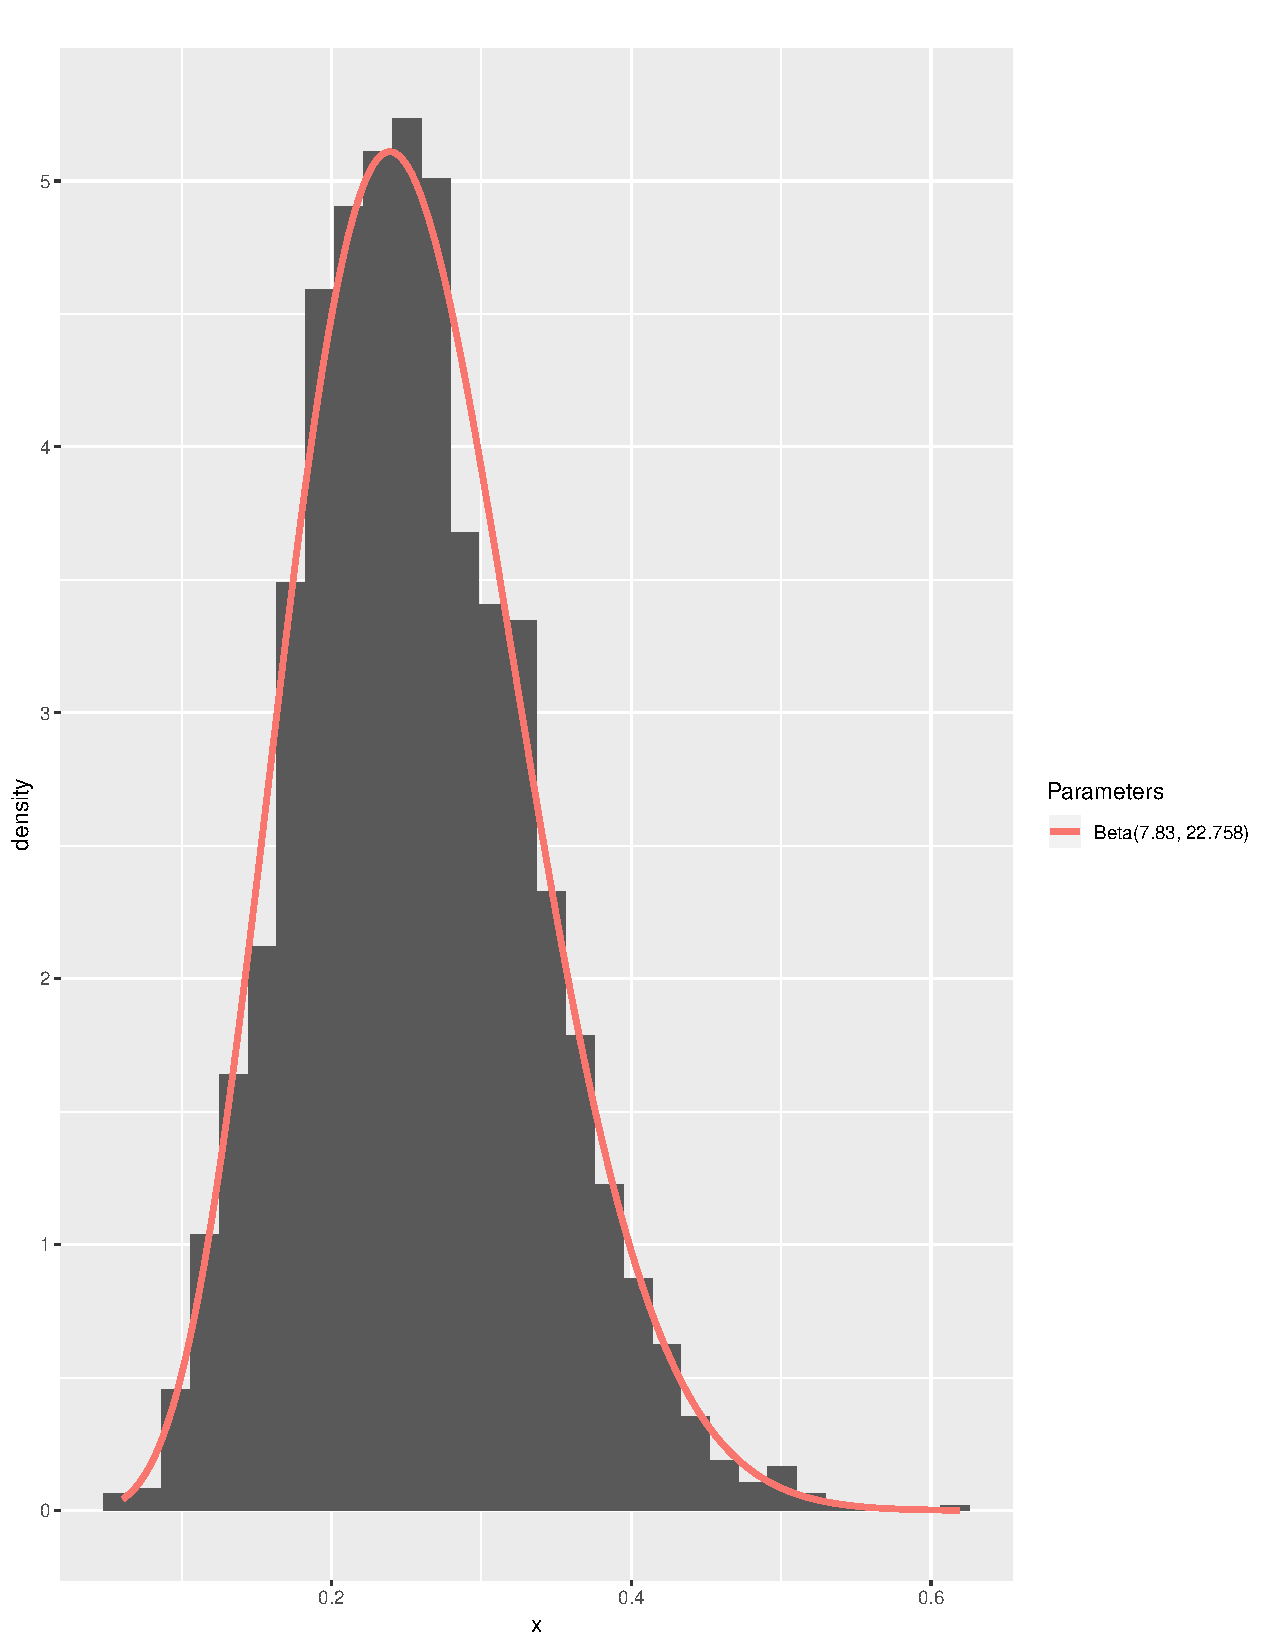
\includegraphics[width = .9\linewidth, height = .7\linewidth]{../../../Figures/paper_19_05/wvn_vegetation.pdf}
    \caption{Similarity between PolSAR data from forest region and -1/4-wave elementary backscatterer}
    \label{fig:fr_wvn}
\end{figure}

\begin{figure}[!ht]
    \centering
    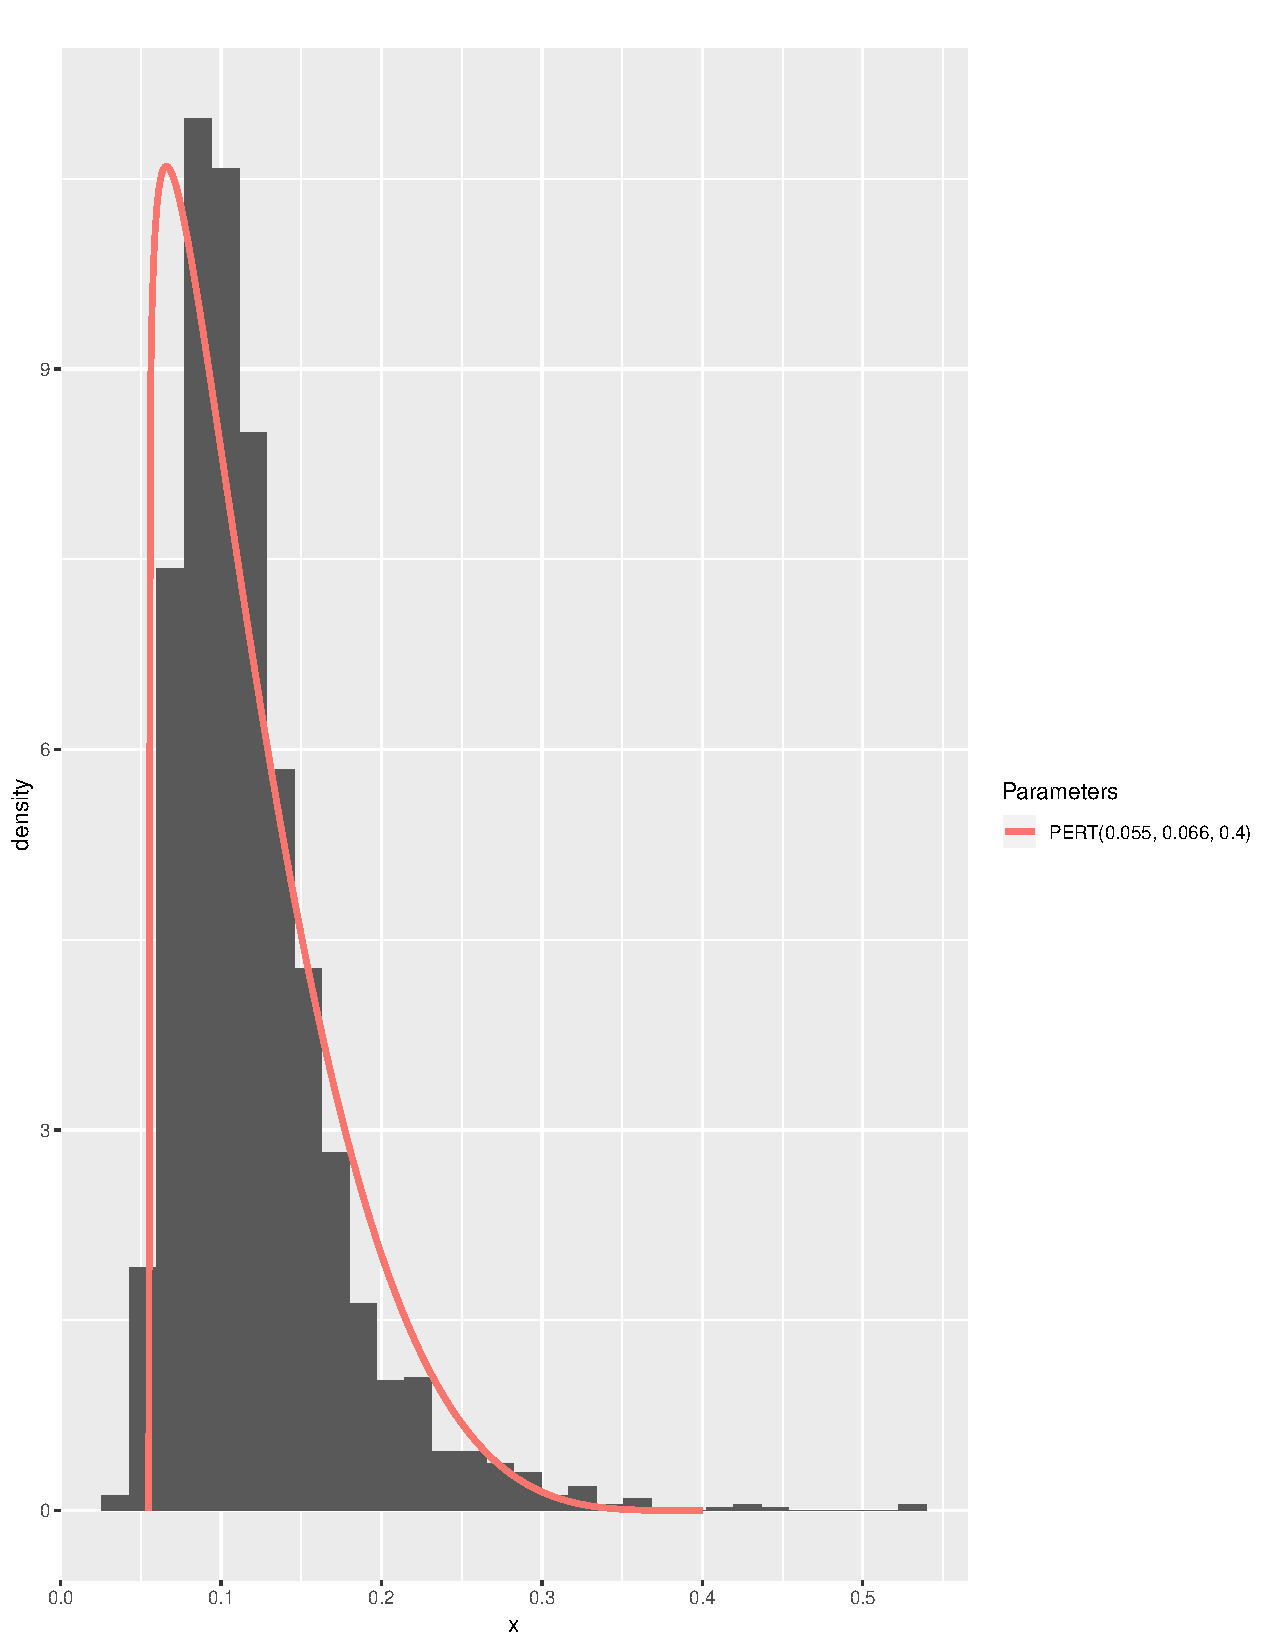
\includegraphics[width = .9\linewidth, height = .7\linewidth]{../../../Figures/paper_19_05/wvn_ground.pdf}
    \caption{Similarity between PolSAR data from ground region and -1/4-wave elementary backscatterer}
    \label{fig:gr_wvn}
\end{figure}

\begin{figure}[!ht]
    \centering
    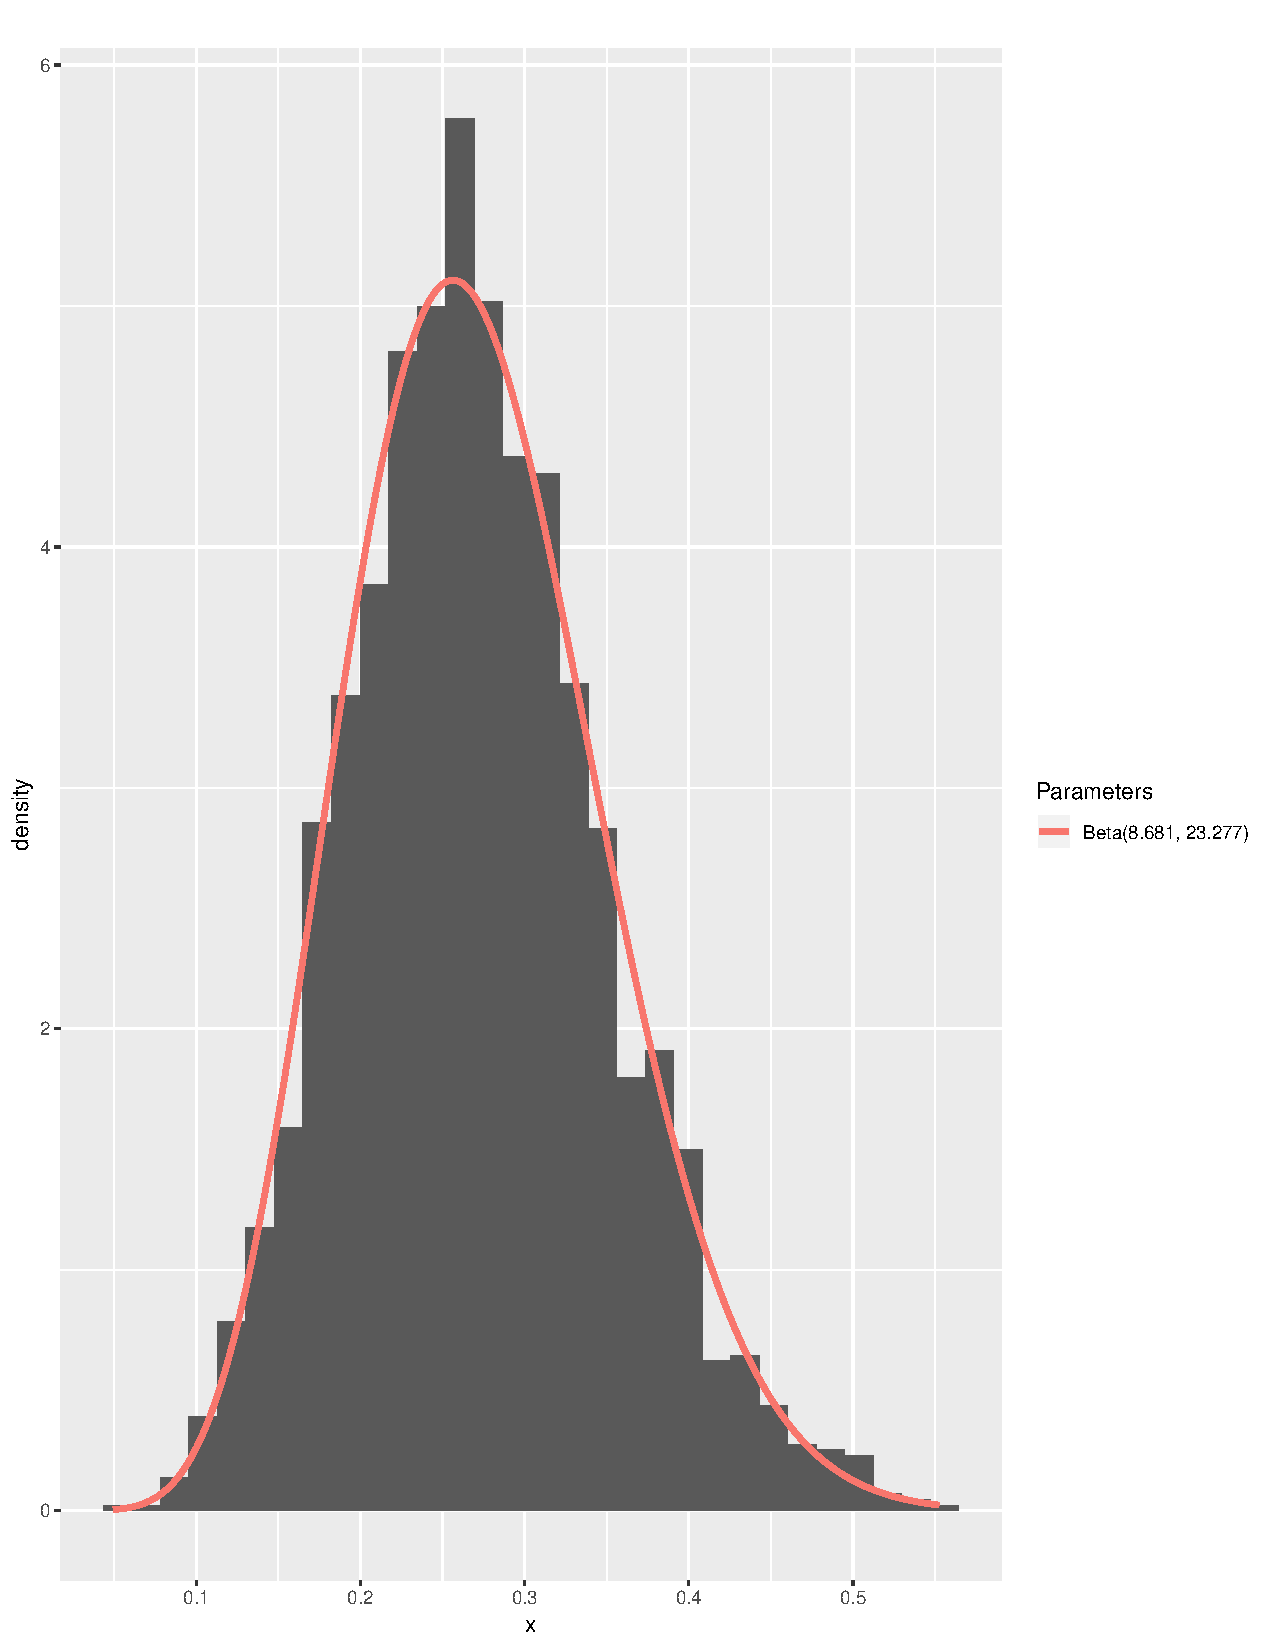
\includegraphics[width = .9\linewidth, height = .7\linewidth]{../../../Figures/paper_19_05/wvp_vegetation.pdf}
    \caption{Similarity between PolSAR data from forest region and +1/4-wave elementary backscatterer}
    \label{fig:fr_wvp}
\end{figure}

\begin{figure}[!ht]
    \centering
    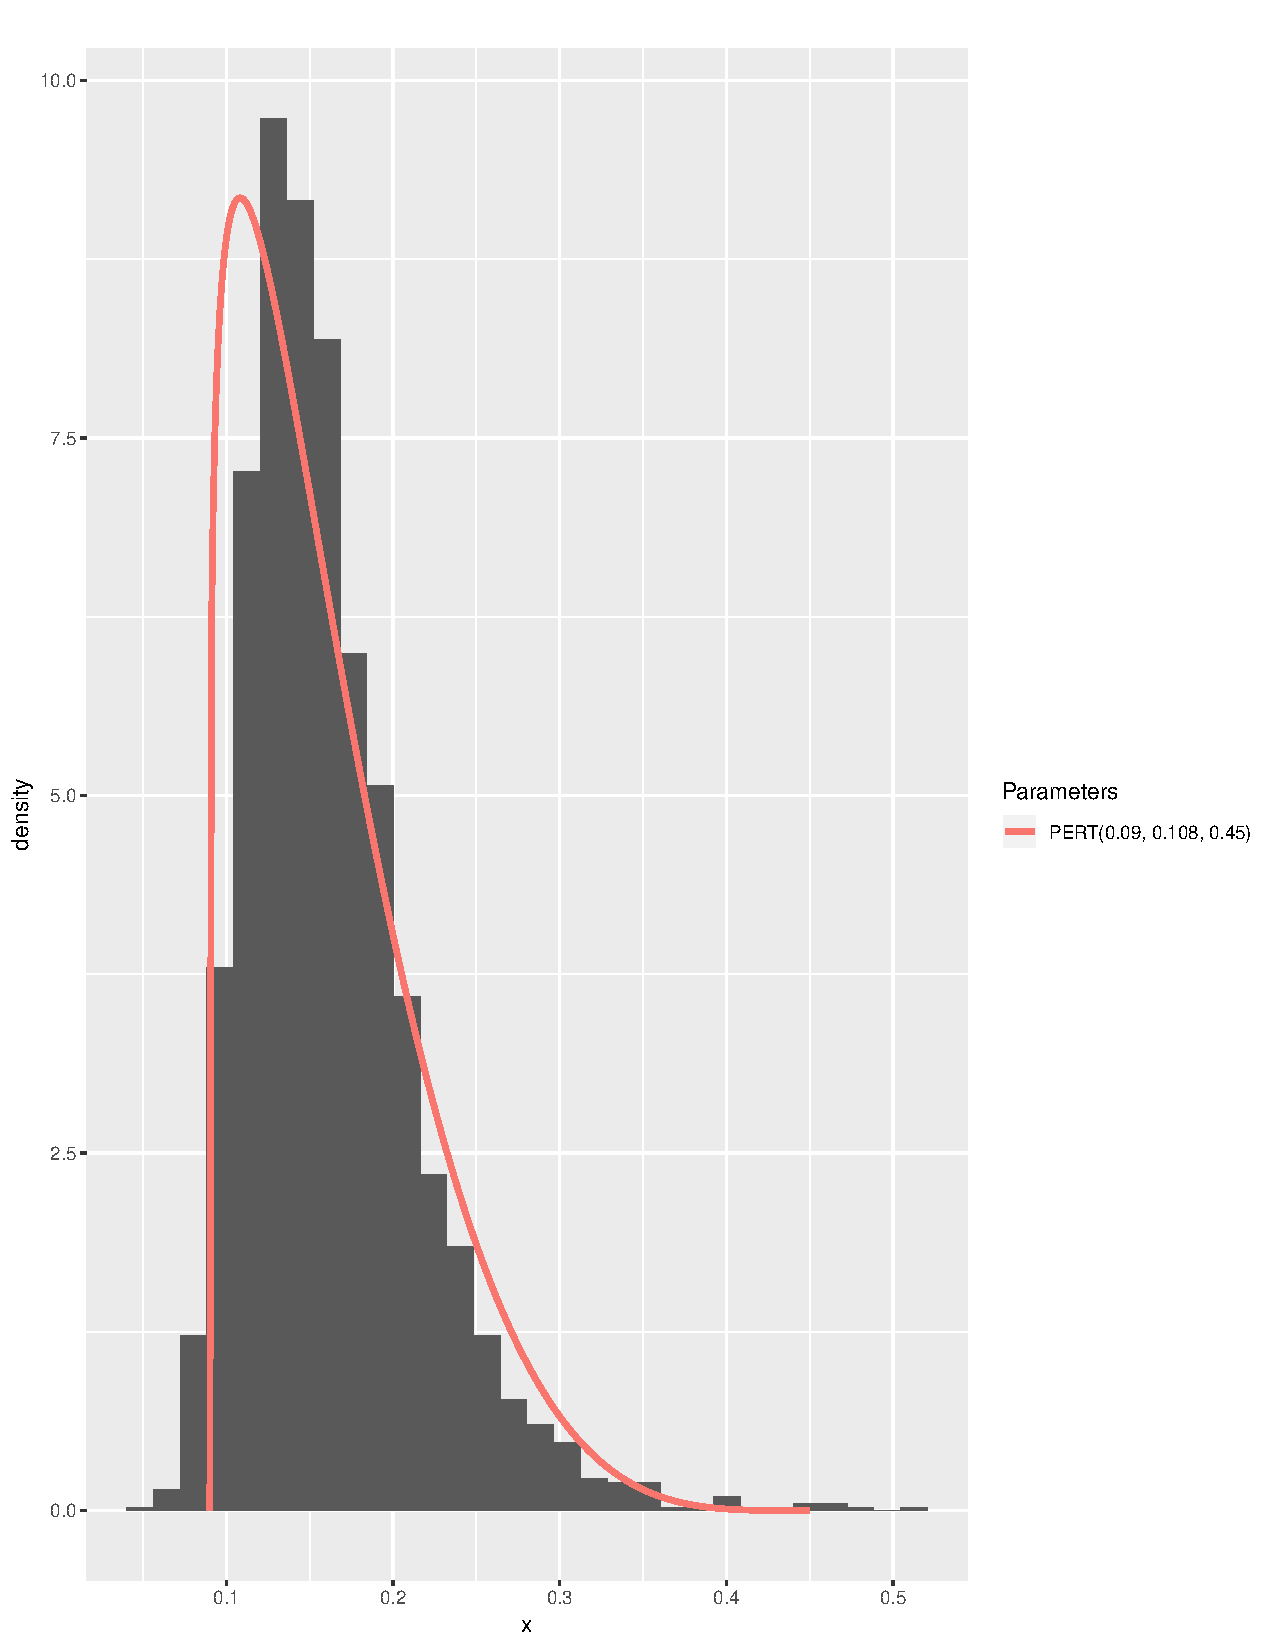
\includegraphics[width = .9\linewidth, height = .7\linewidth]{../../../Figures/paper_19_05/wvp_ground.pdf}
    \caption{Similarity between PolSAR data from ground region and +1/4-wave elementary backscatterer}
    \label{fig:gr_wvp}
\end{figure}

\begin{figure}[!ht]
    \centering
    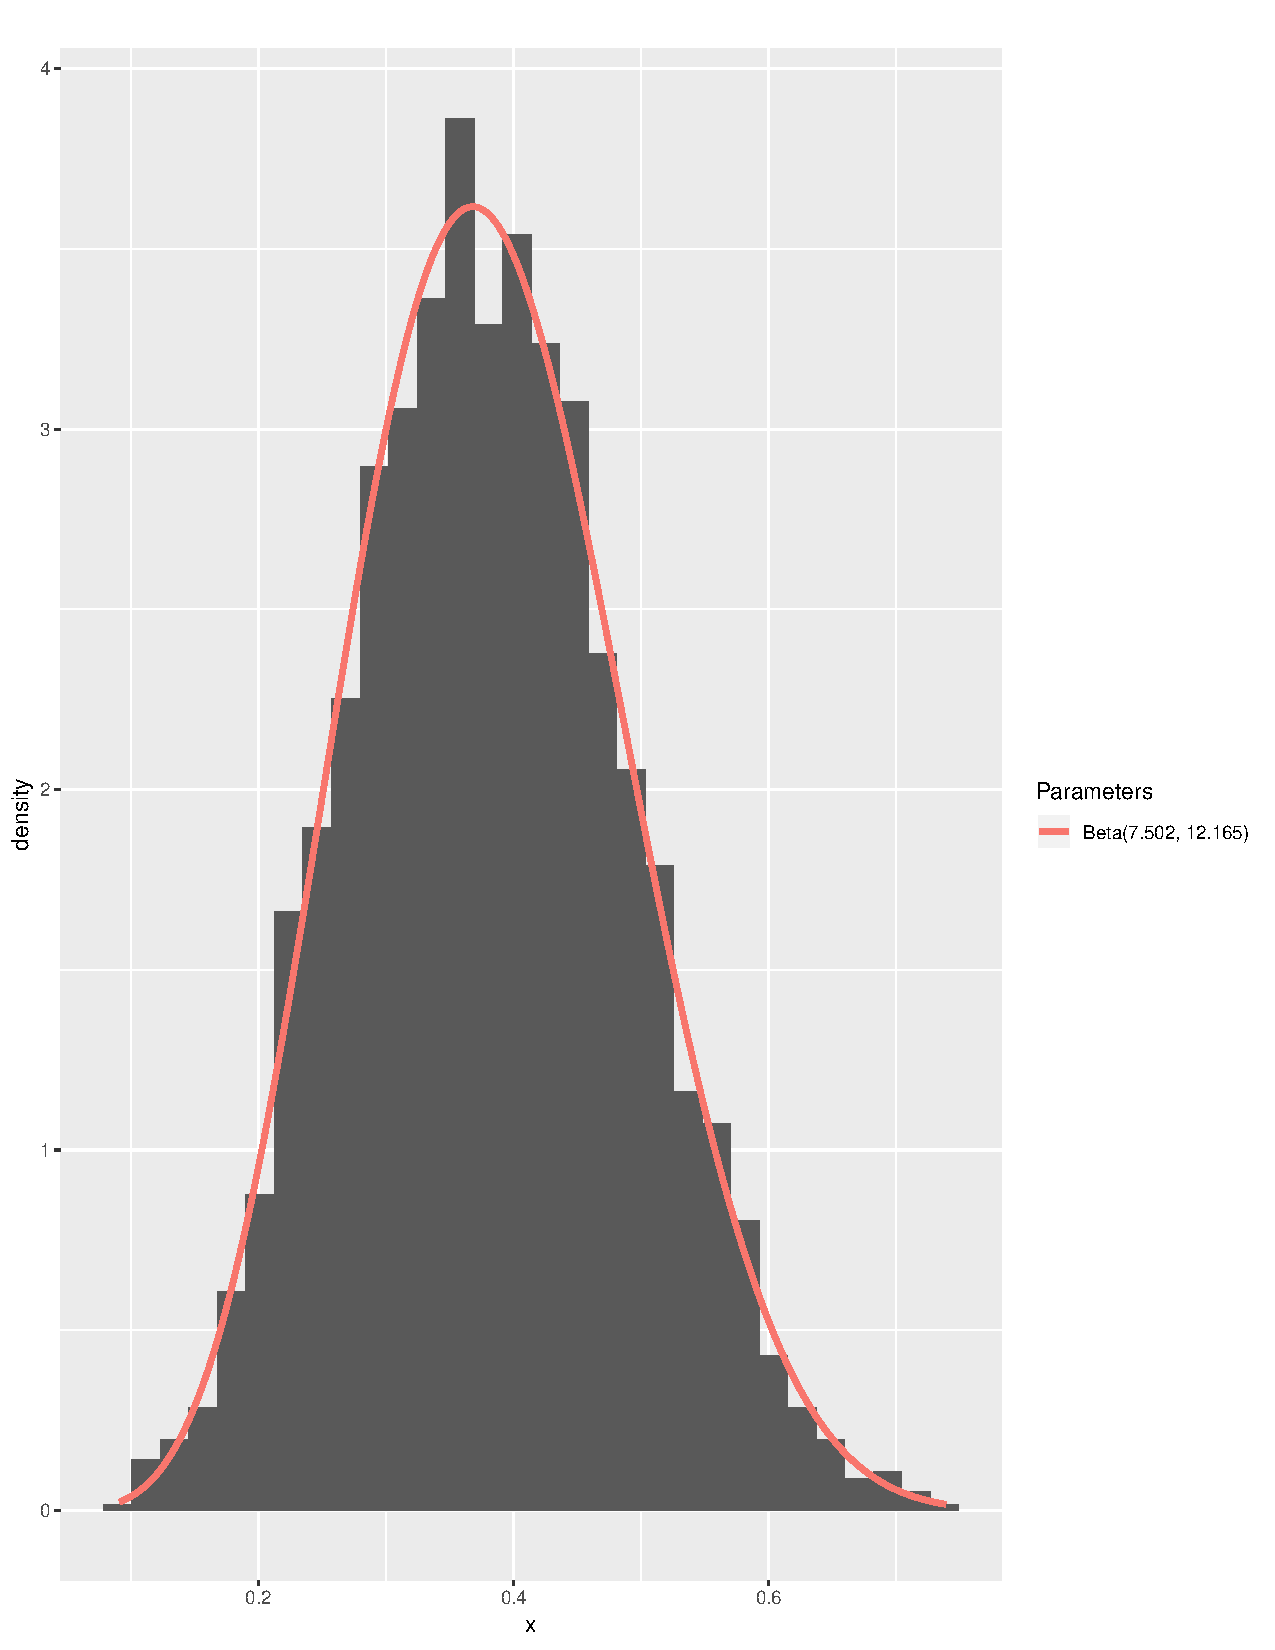
\includegraphics[width = .9\linewidth, height = .7\linewidth]{../../../Figures/paper_19_05/cy_vegetation.pdf}
    \caption{Similarity between PolSAR data from forest region and cylinder elementary backscatterer}
    \label{fig:fr_cy}
\end{figure}

\begin{figure}[!ht]
    \centering
    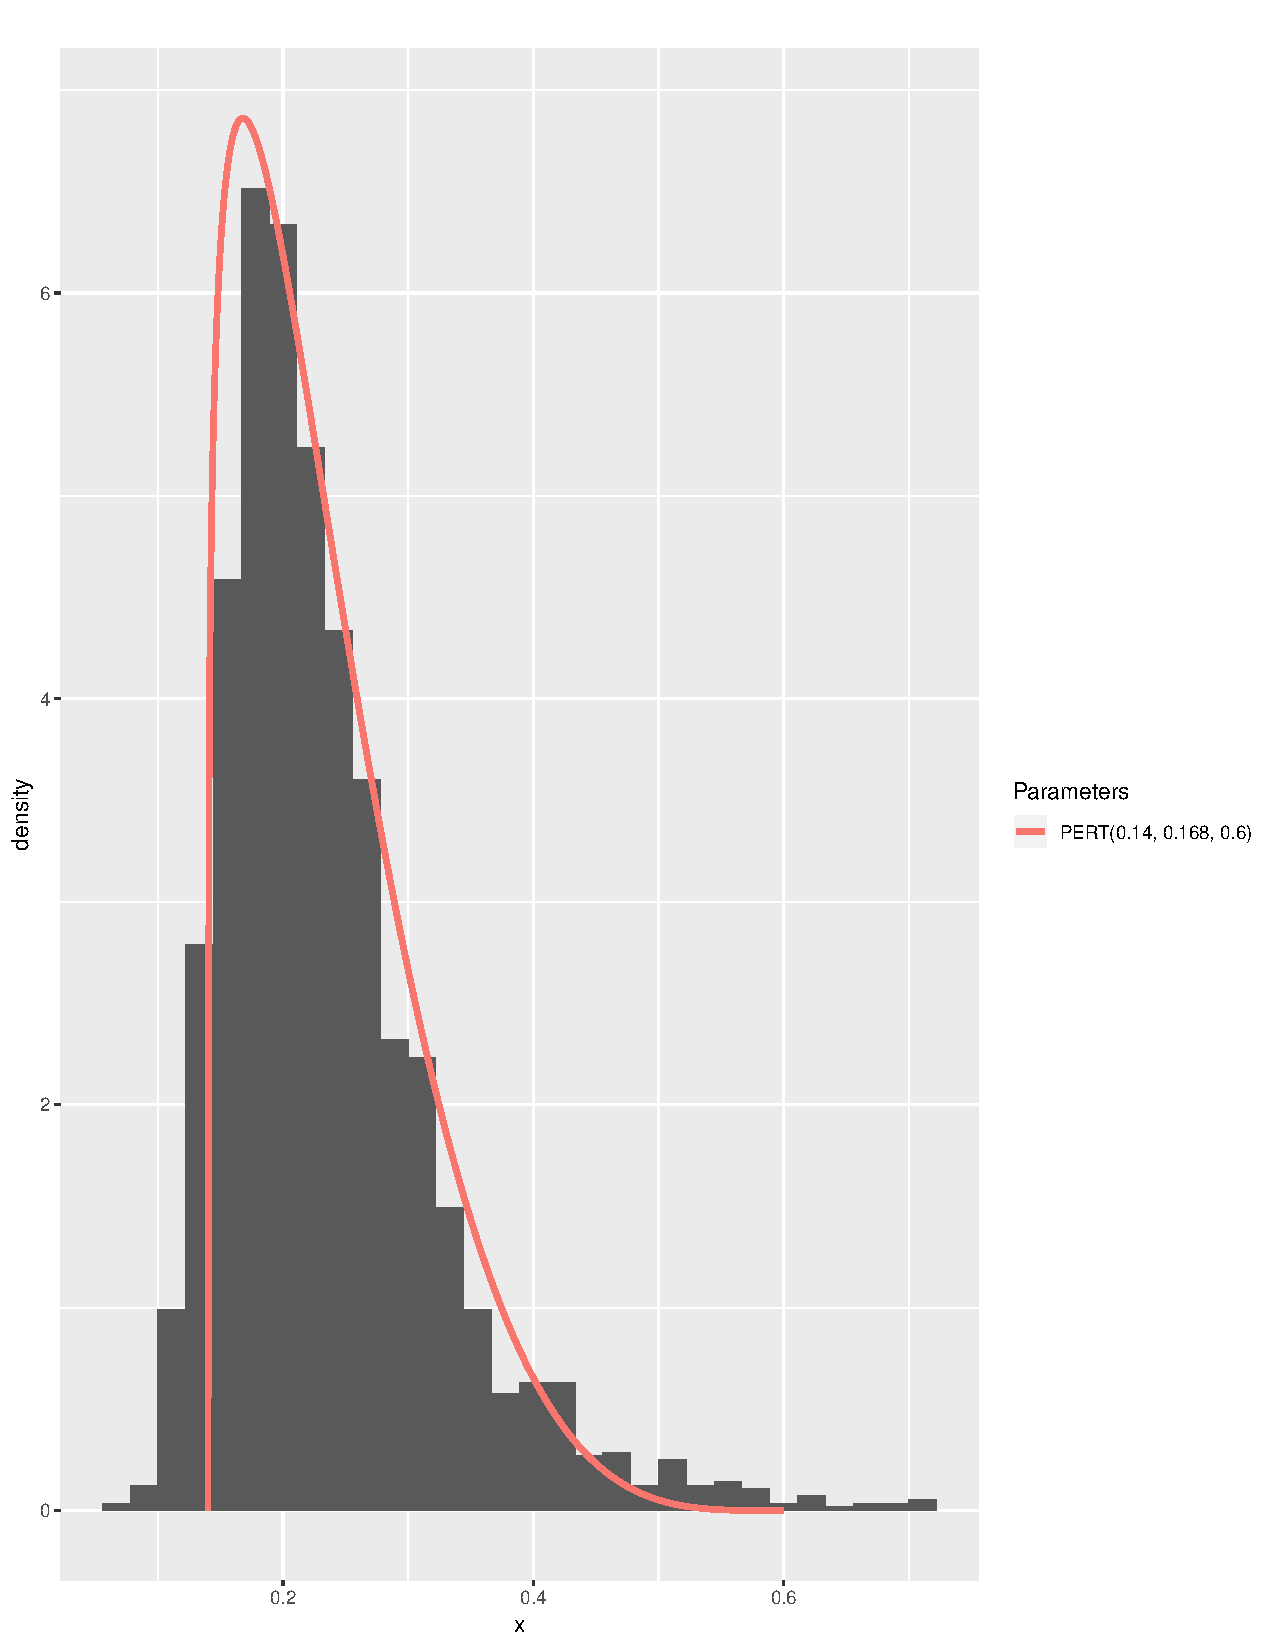
\includegraphics[width = .9\linewidth, height = .7\linewidth]{../../../Figures/paper_19_05/cy_ground.pdf}
    \caption{Similarity between PolSAR data from ground region and cylinder elementary backscatterer}
    \label{fig:gr_cy}
\end{figure}

\begin{figure}[!ht]
    \centering
    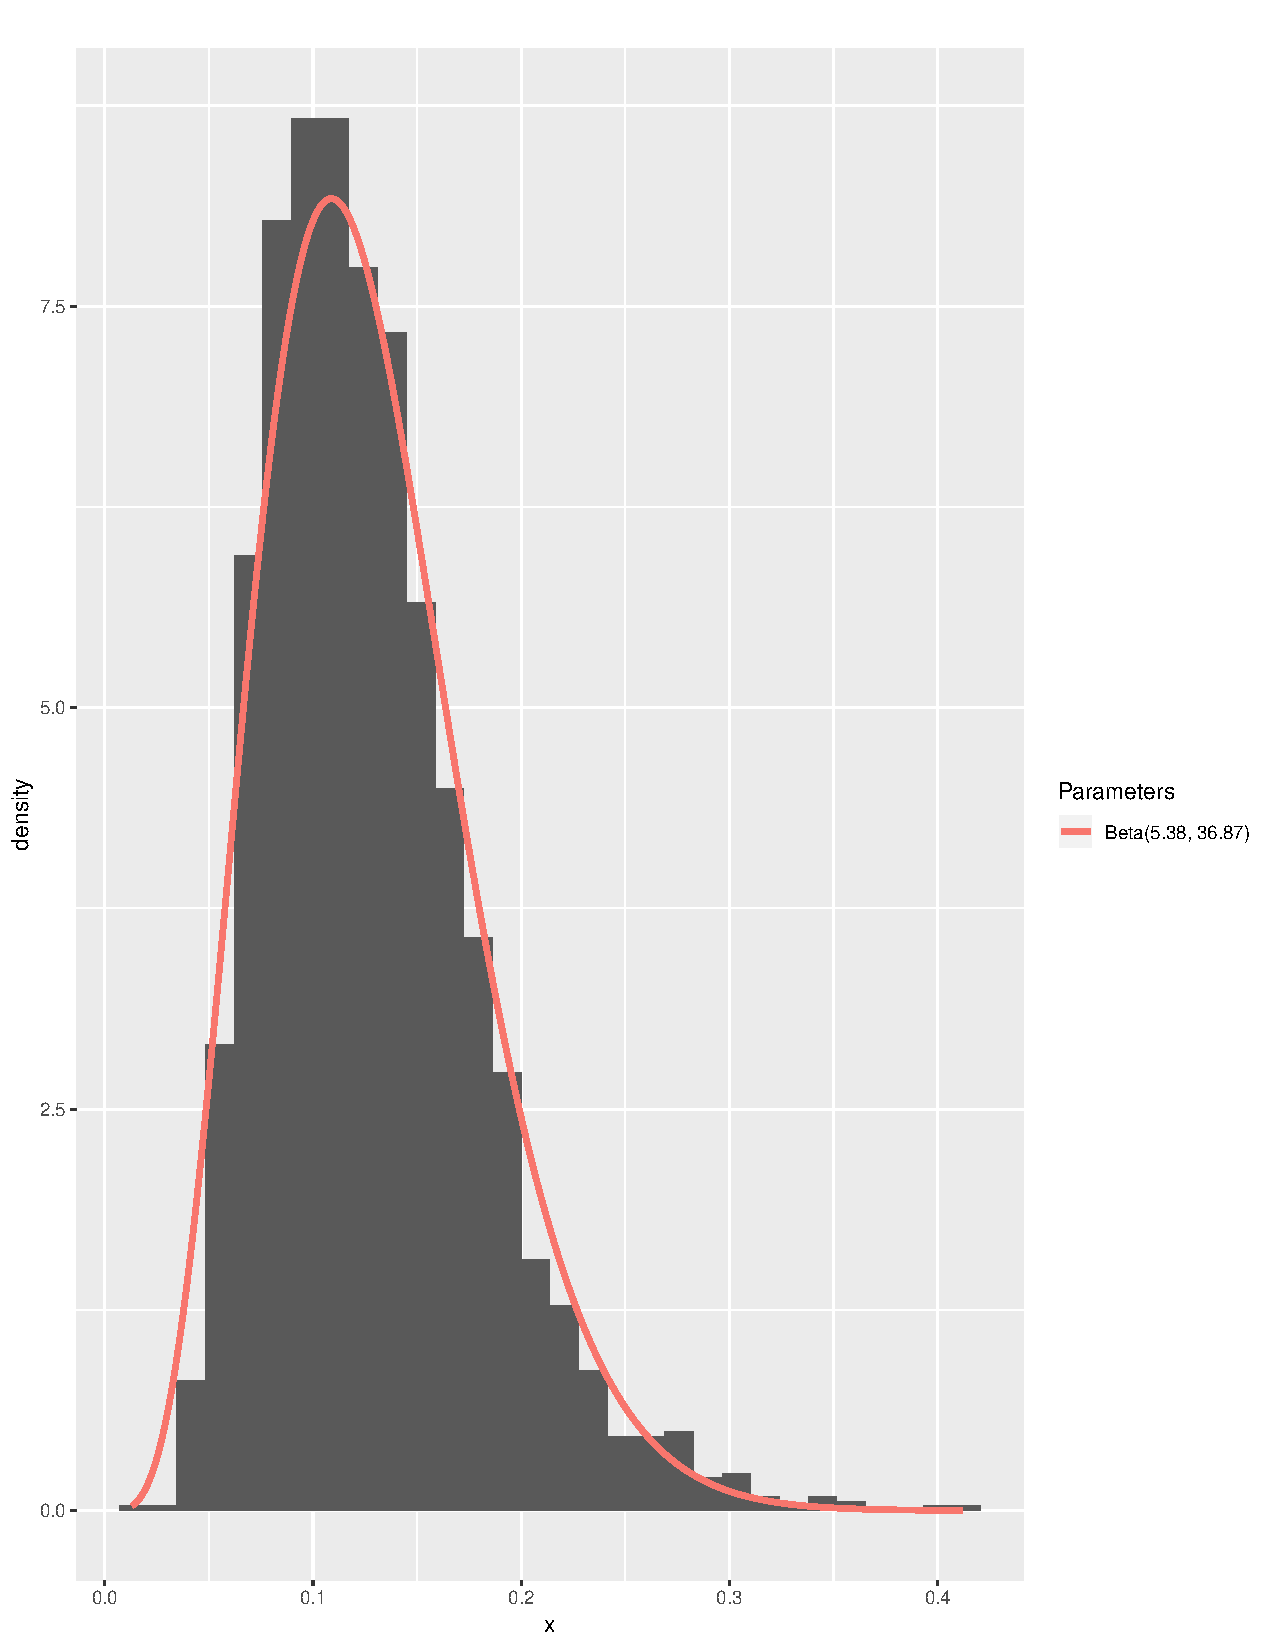
\includegraphics[width = .9\linewidth, height = .7\linewidth]{../../../Figures/paper_19_05/di_vegetation.pdf}
    \caption{Similarity between PolSAR data from forest region and dihedral elementary backscatterer}
    \label{fig:fr_di}
\end{figure}

\begin{figure}[!ht]
    \centering
    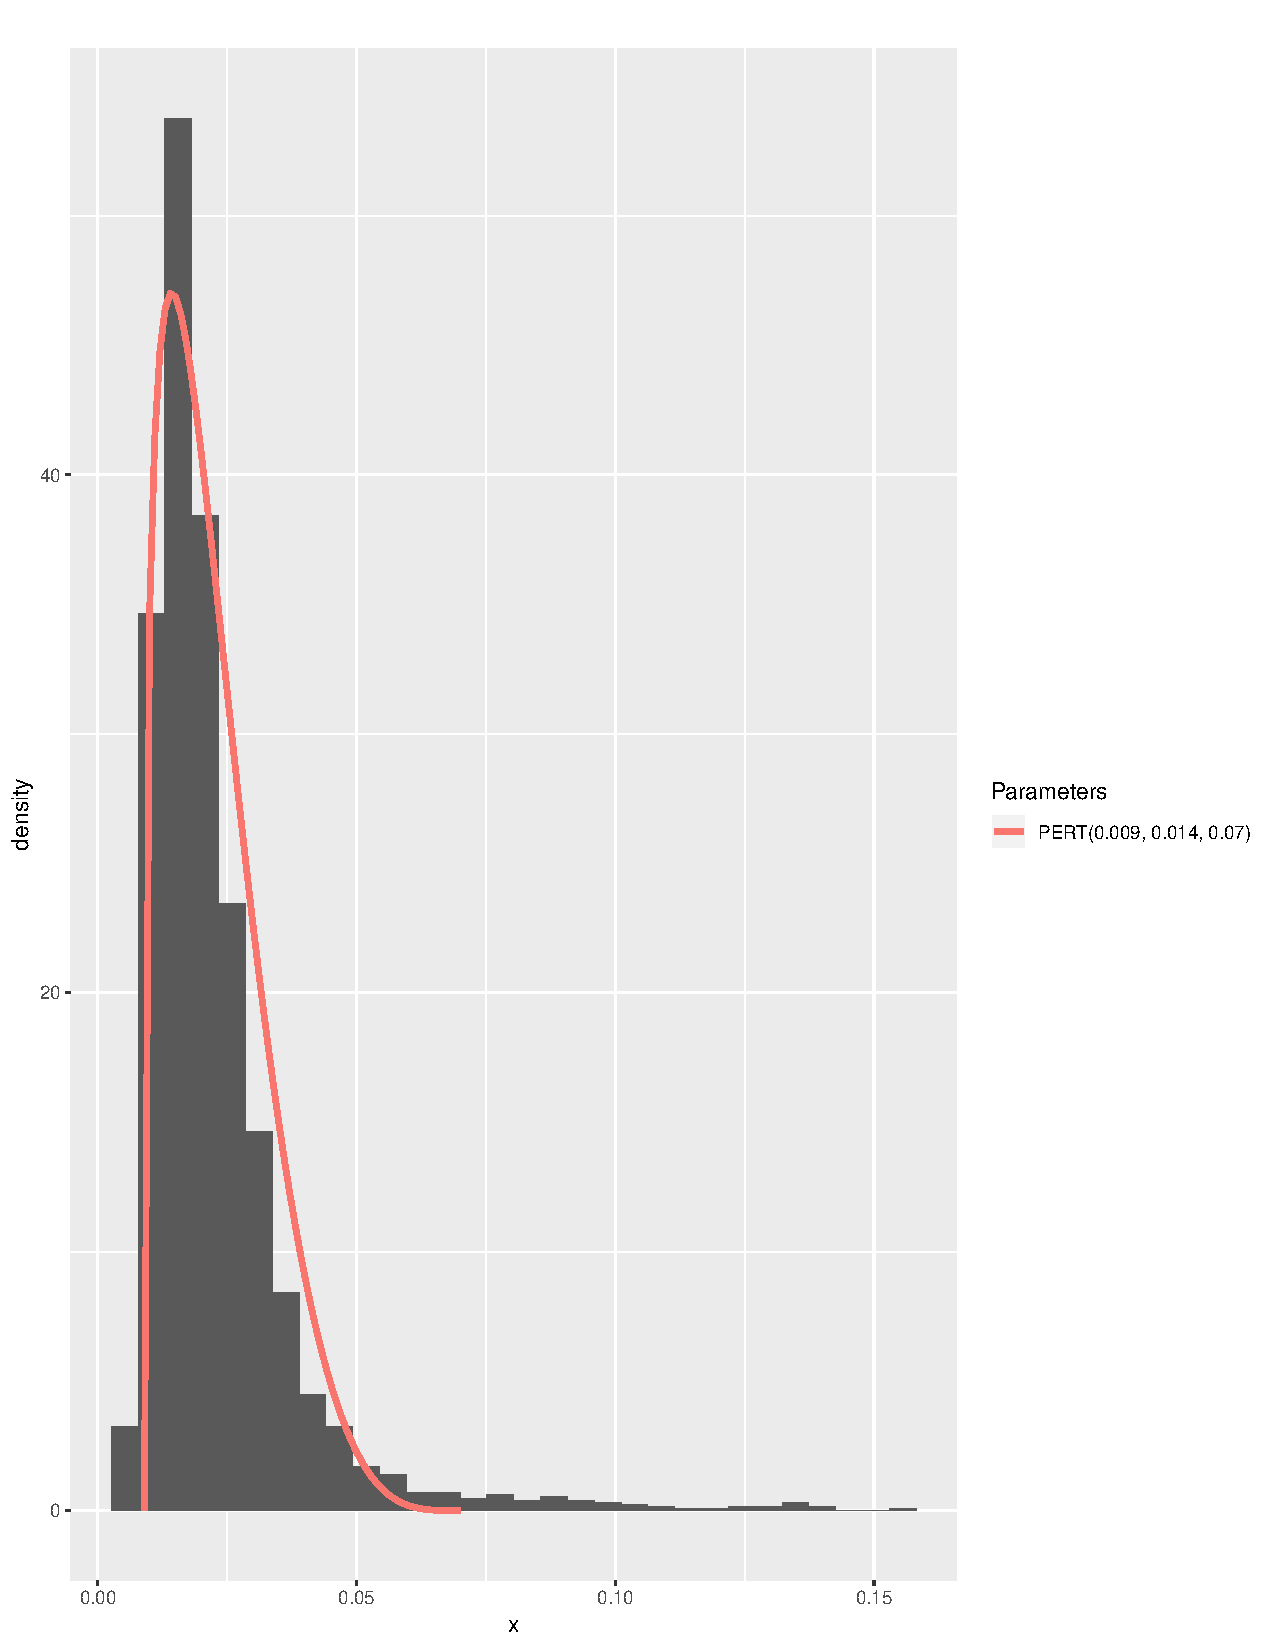
\includegraphics[width = .9\linewidth, height = .7\linewidth]{../../../Figures/paper_19_05/di_ground.pdf}
    \caption{Similarity between PolSAR data from ground region and dihedral elementary backscatterer}
    \label{fig:gr_di}
\end{figure}

\begin{figure}[!ht]
    \centering
    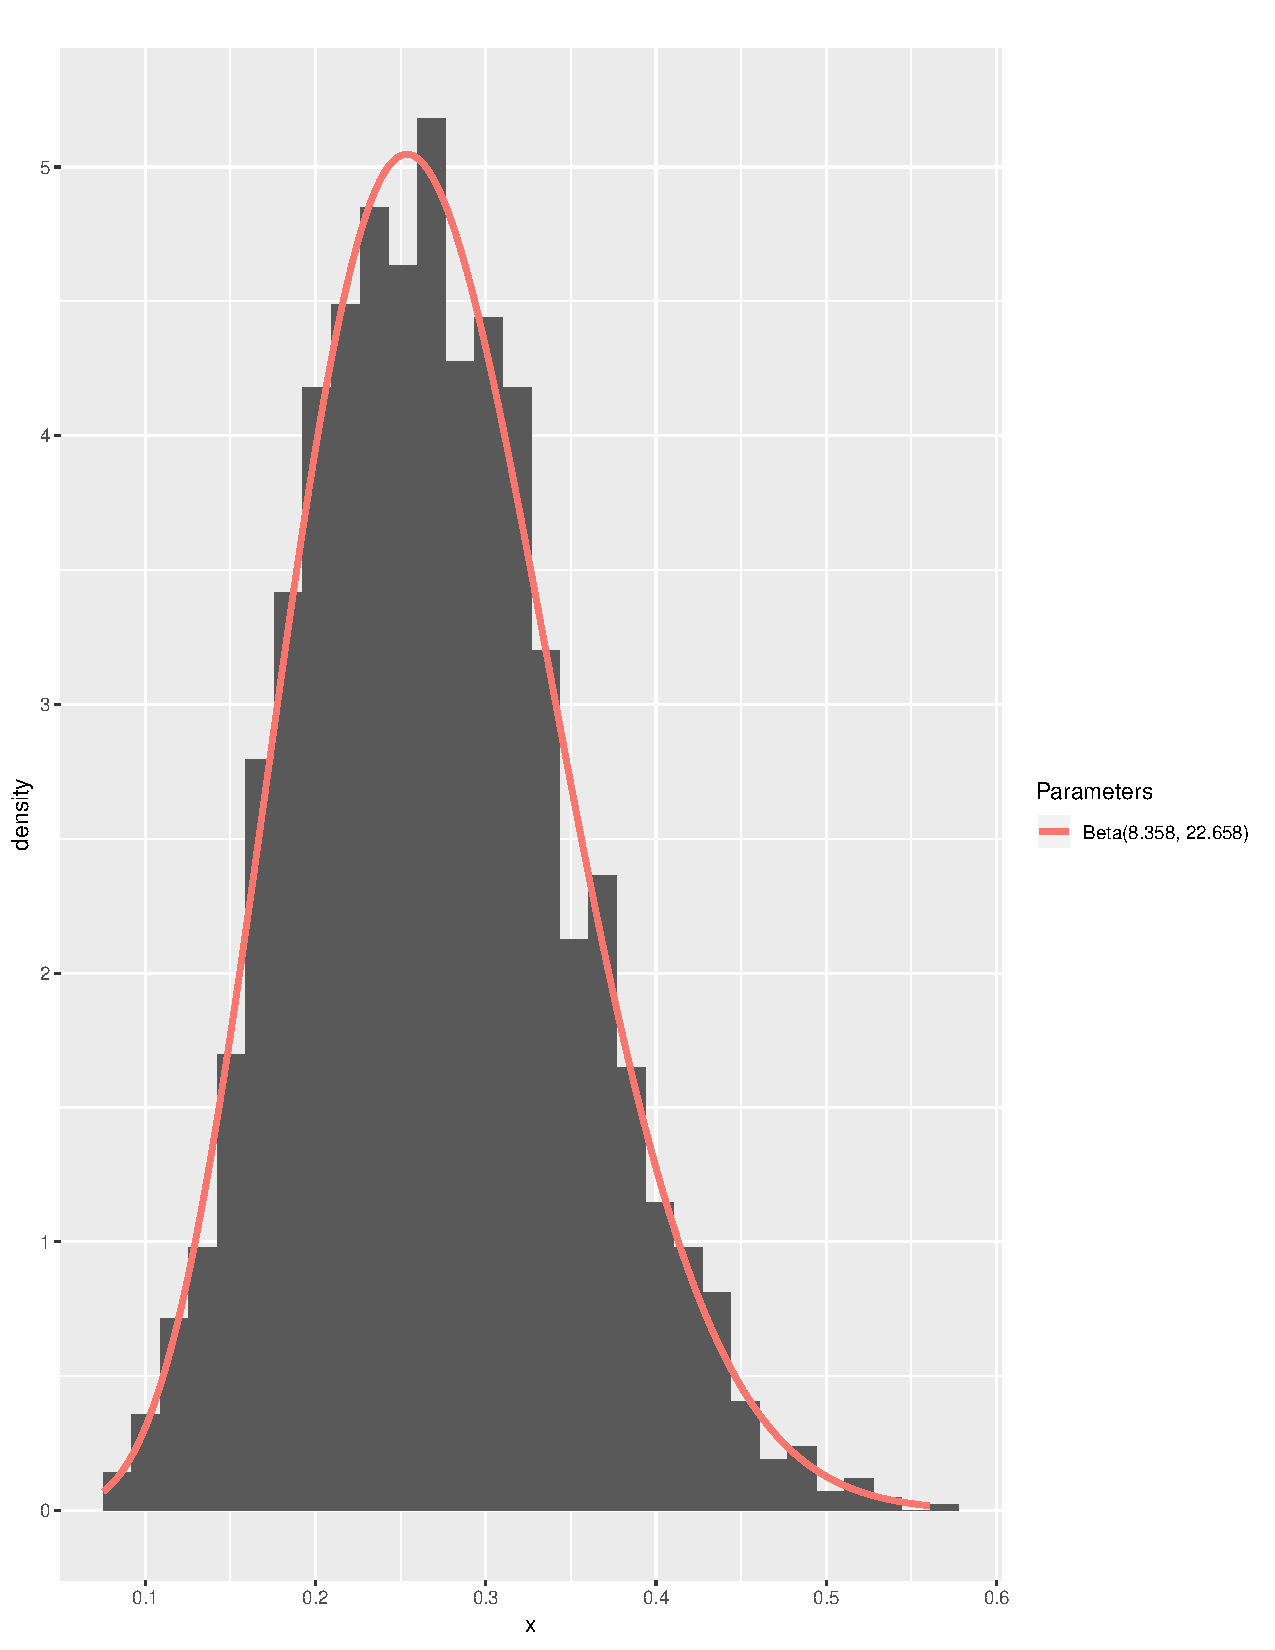
\includegraphics[width = .9\linewidth, height = .7\linewidth]{../../../Figures/paper_19_05/dip_vegetation.pdf}
    \caption{Similarity between PolSAR data from forest region and dipole elementary backscatterer}
    \label{fig:fr_dip}
\end{figure}

\begin{figure}[!ht]
    \centering
    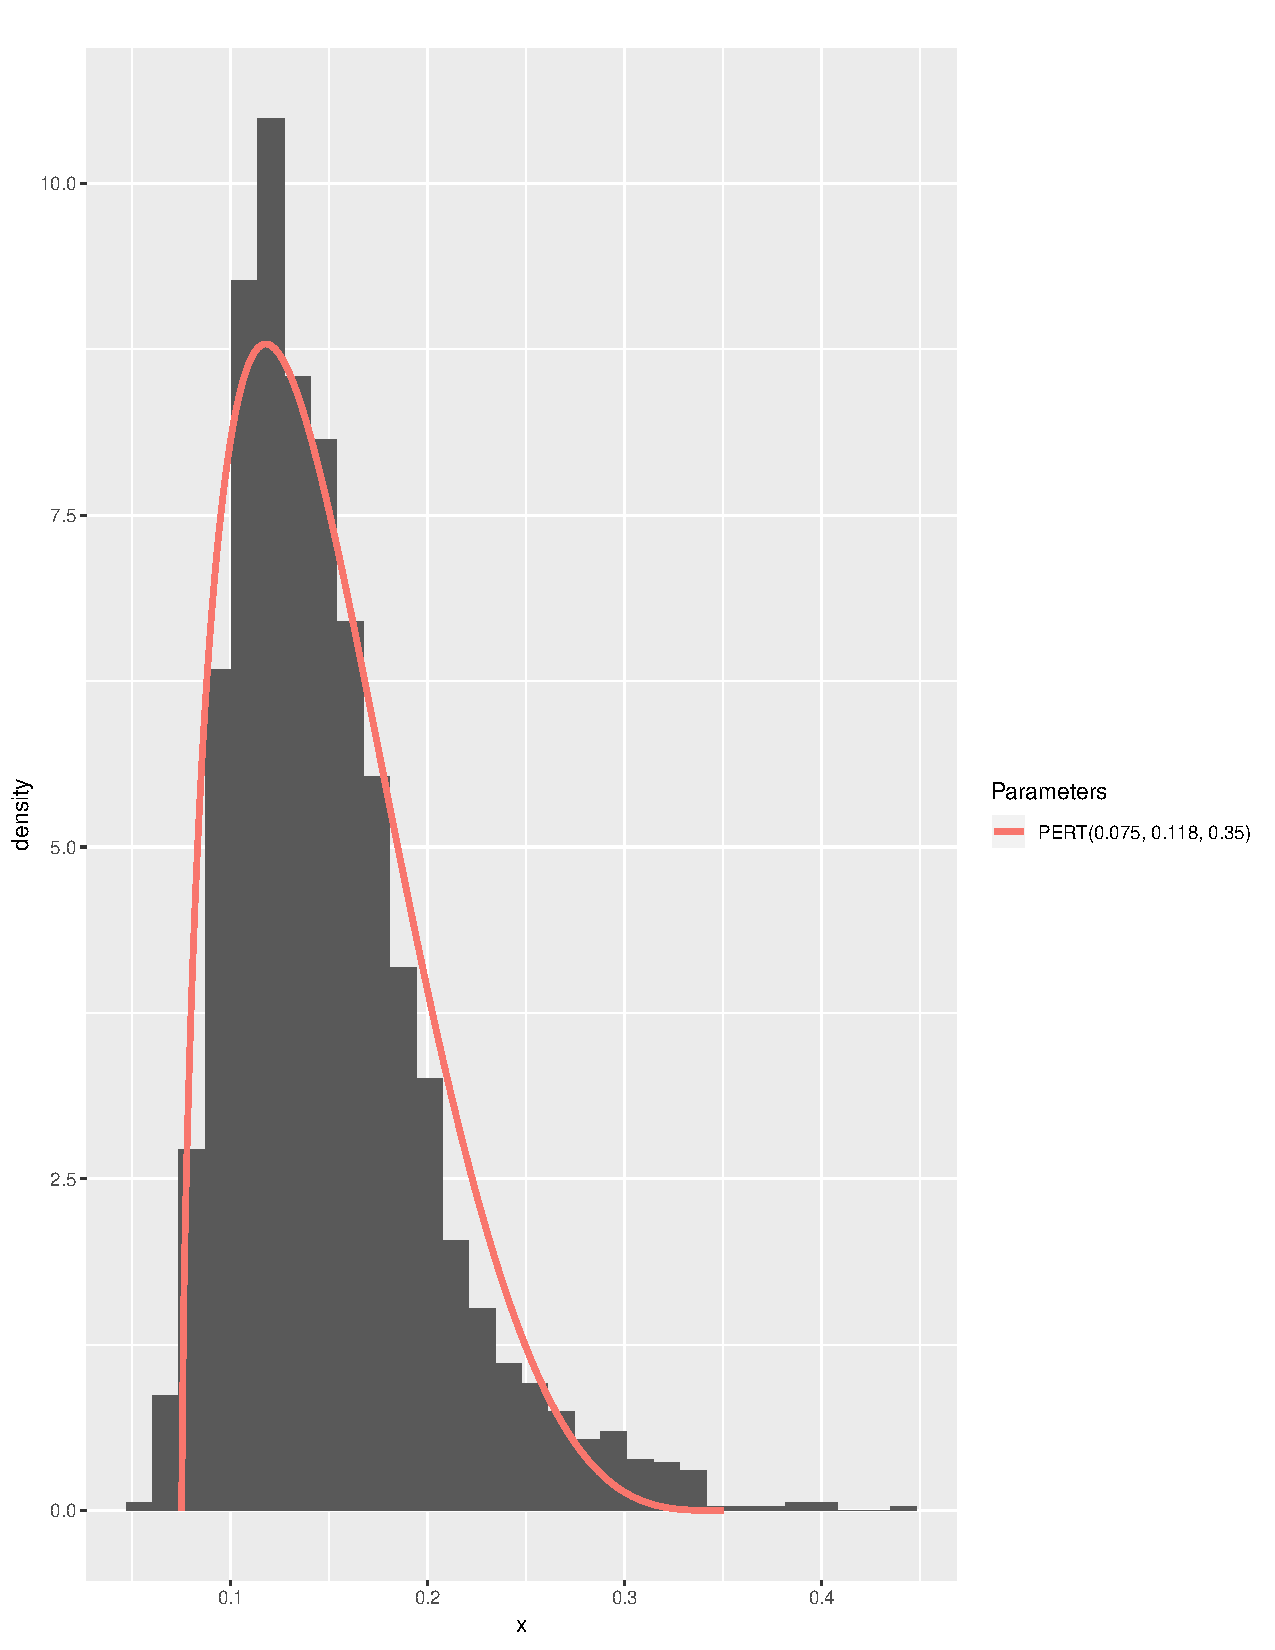
\includegraphics[width = .9\linewidth, height = .7\linewidth]{../../../Figures/paper_19_05/dip_ground.pdf}
    \caption{Similarity between PolSAR data from ground region and dipole elementary backscatterer}
    \label{fig:gr_dip}
\end{figure}

\begin{figure}[!ht]
    \centering
    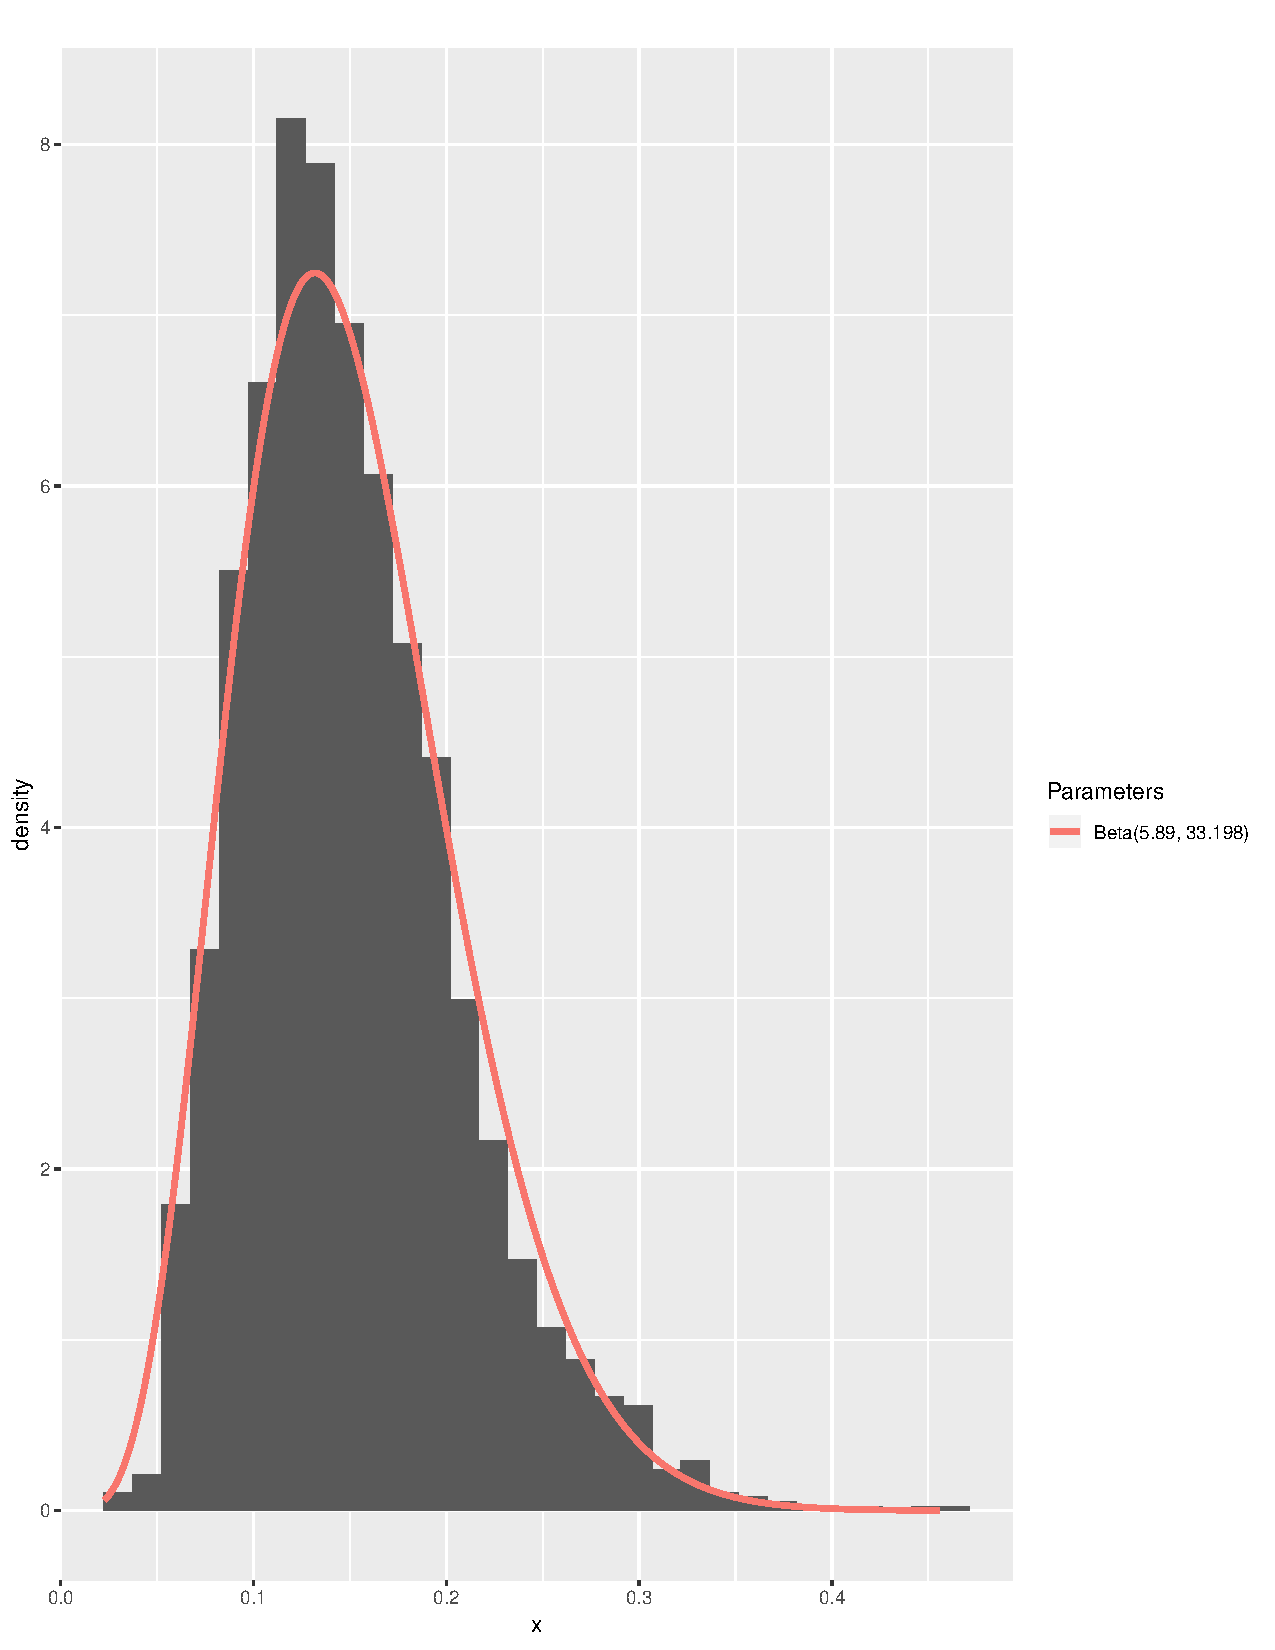
\includegraphics[width = .9\linewidth, height = .7\linewidth]{../../../Figures/paper_19_05/nd_vegetation.pdf}
    \caption{Similarity between PolSAR data from forest region and narrow dihedral elementary backscatterer}
    \label{fig:fr_nd}
\end{figure}

\begin{figure}[!ht]
    \centering
    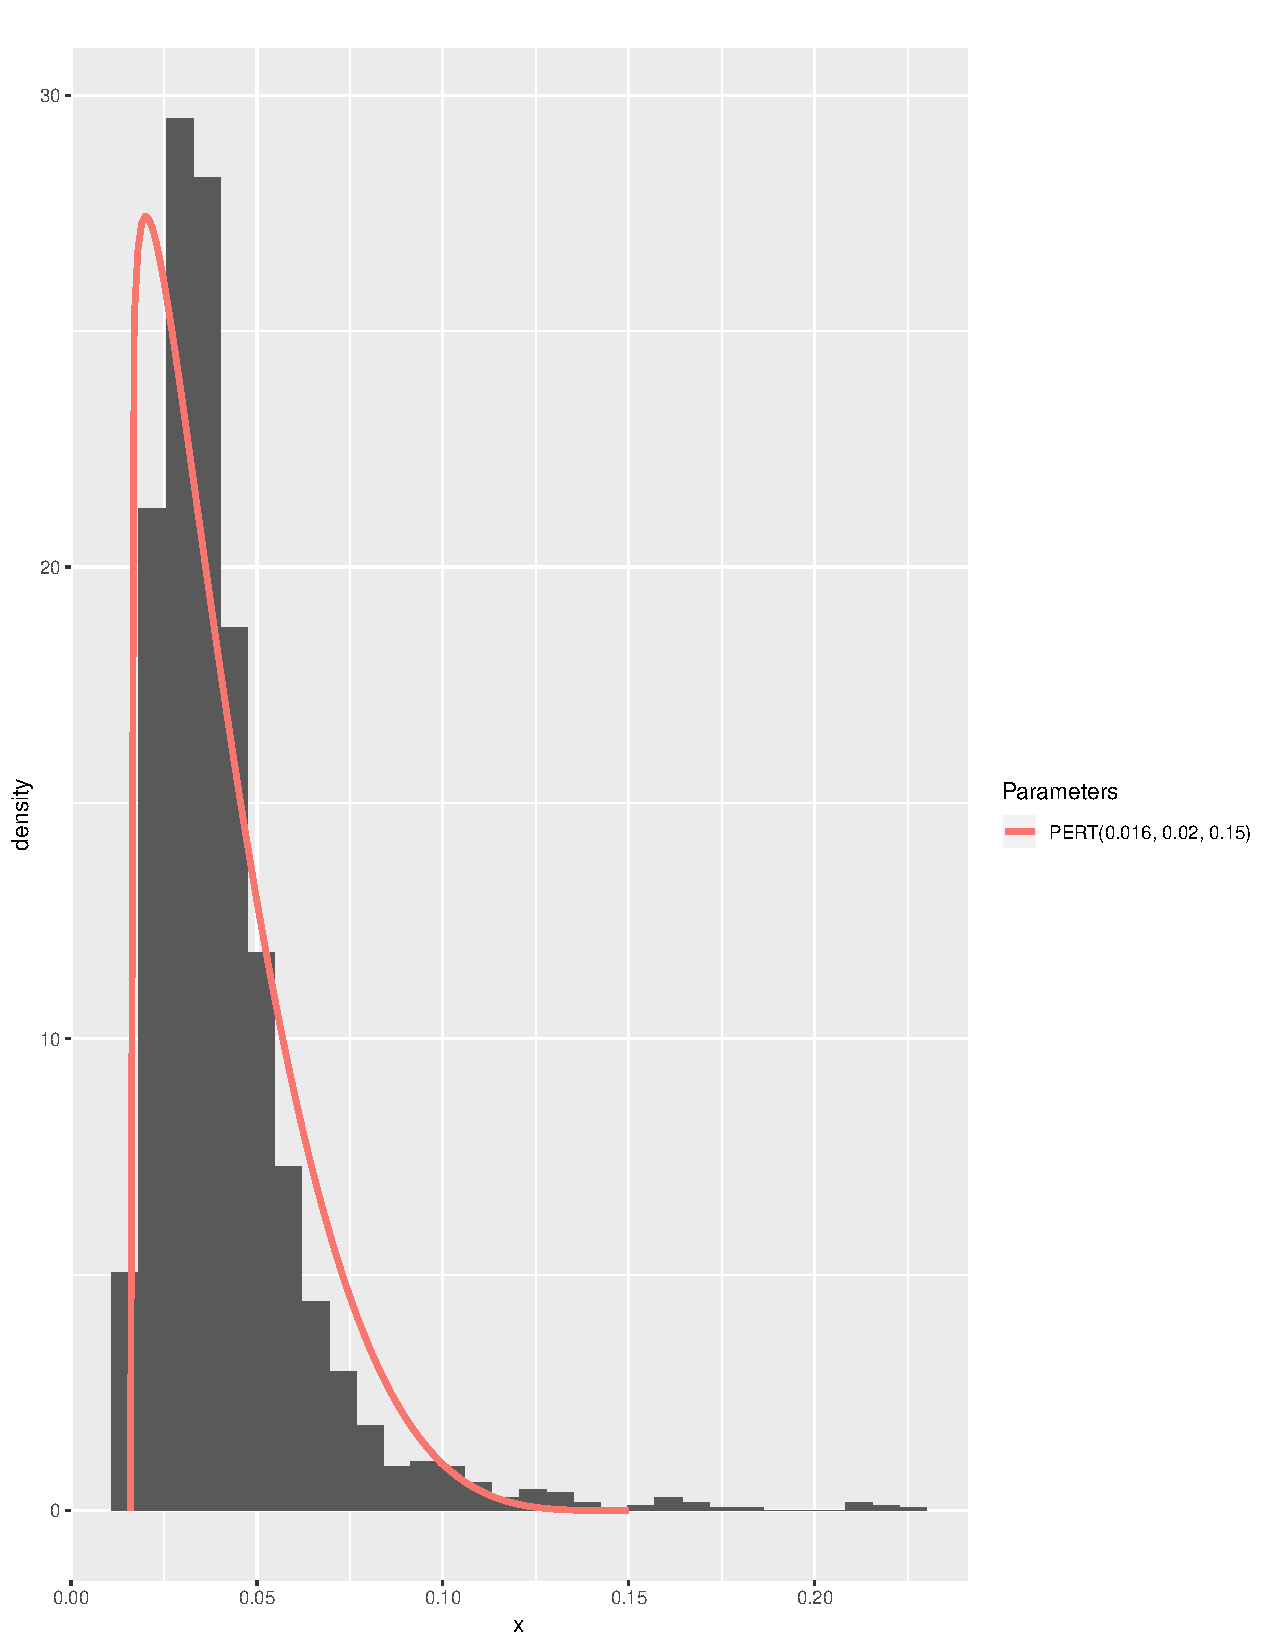
\includegraphics[width = .9\linewidth, height = .7\linewidth]{../../../Figures/paper_19_05/nd_ground.pdf}
    \caption{Similarity between PolSAR data from ground region and narrow dihedral elementary backscatterer}
    \label{fig:gr_nd}
\end{figure}

\begin{figure}[!ht]
    \centering
    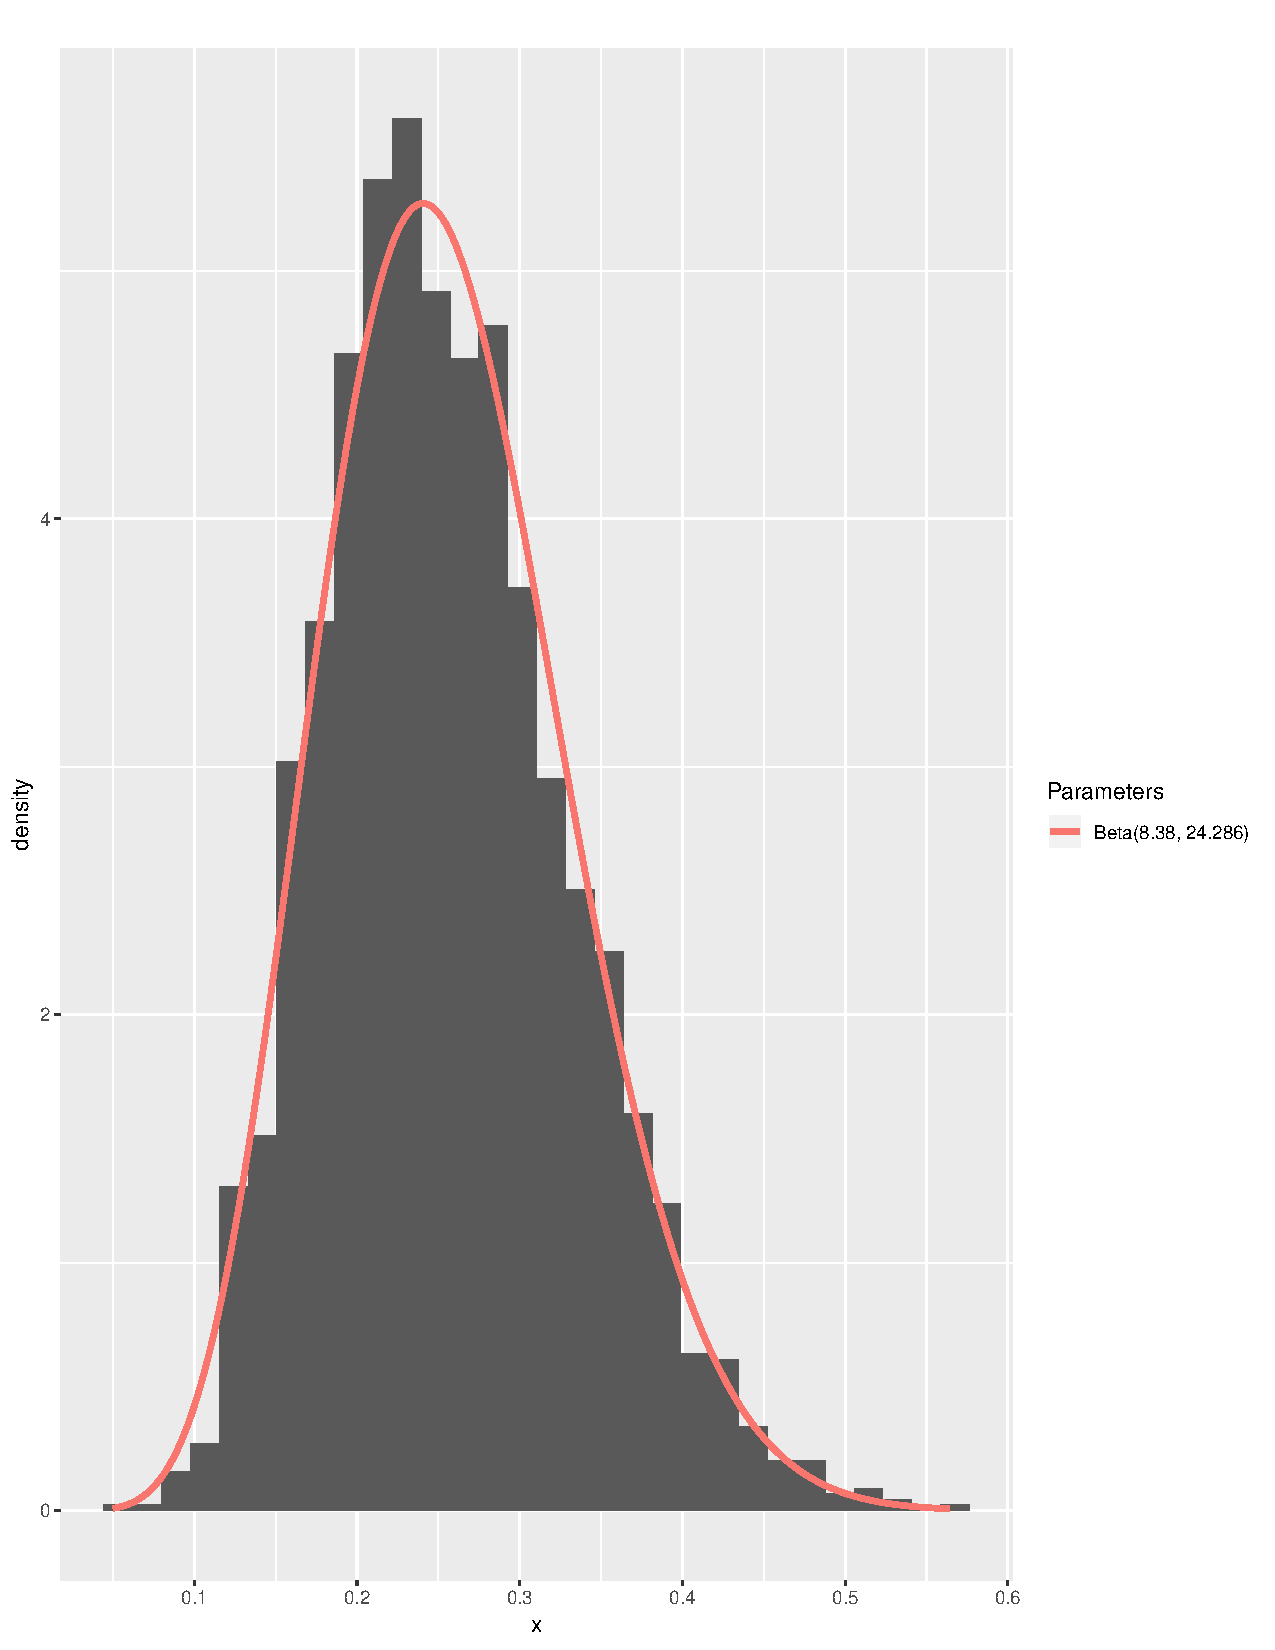
\includegraphics[width = .9\linewidth, height = .7\linewidth]{../../../Figures/paper_19_05/lh_vegetation.pdf}
    \caption{Similarity between PolSAR data from forest region and left helix elementary backscatterer}
    \label{fig:fr_lh}
\end{figure}

\begin{figure}[!ht]
    \centering
    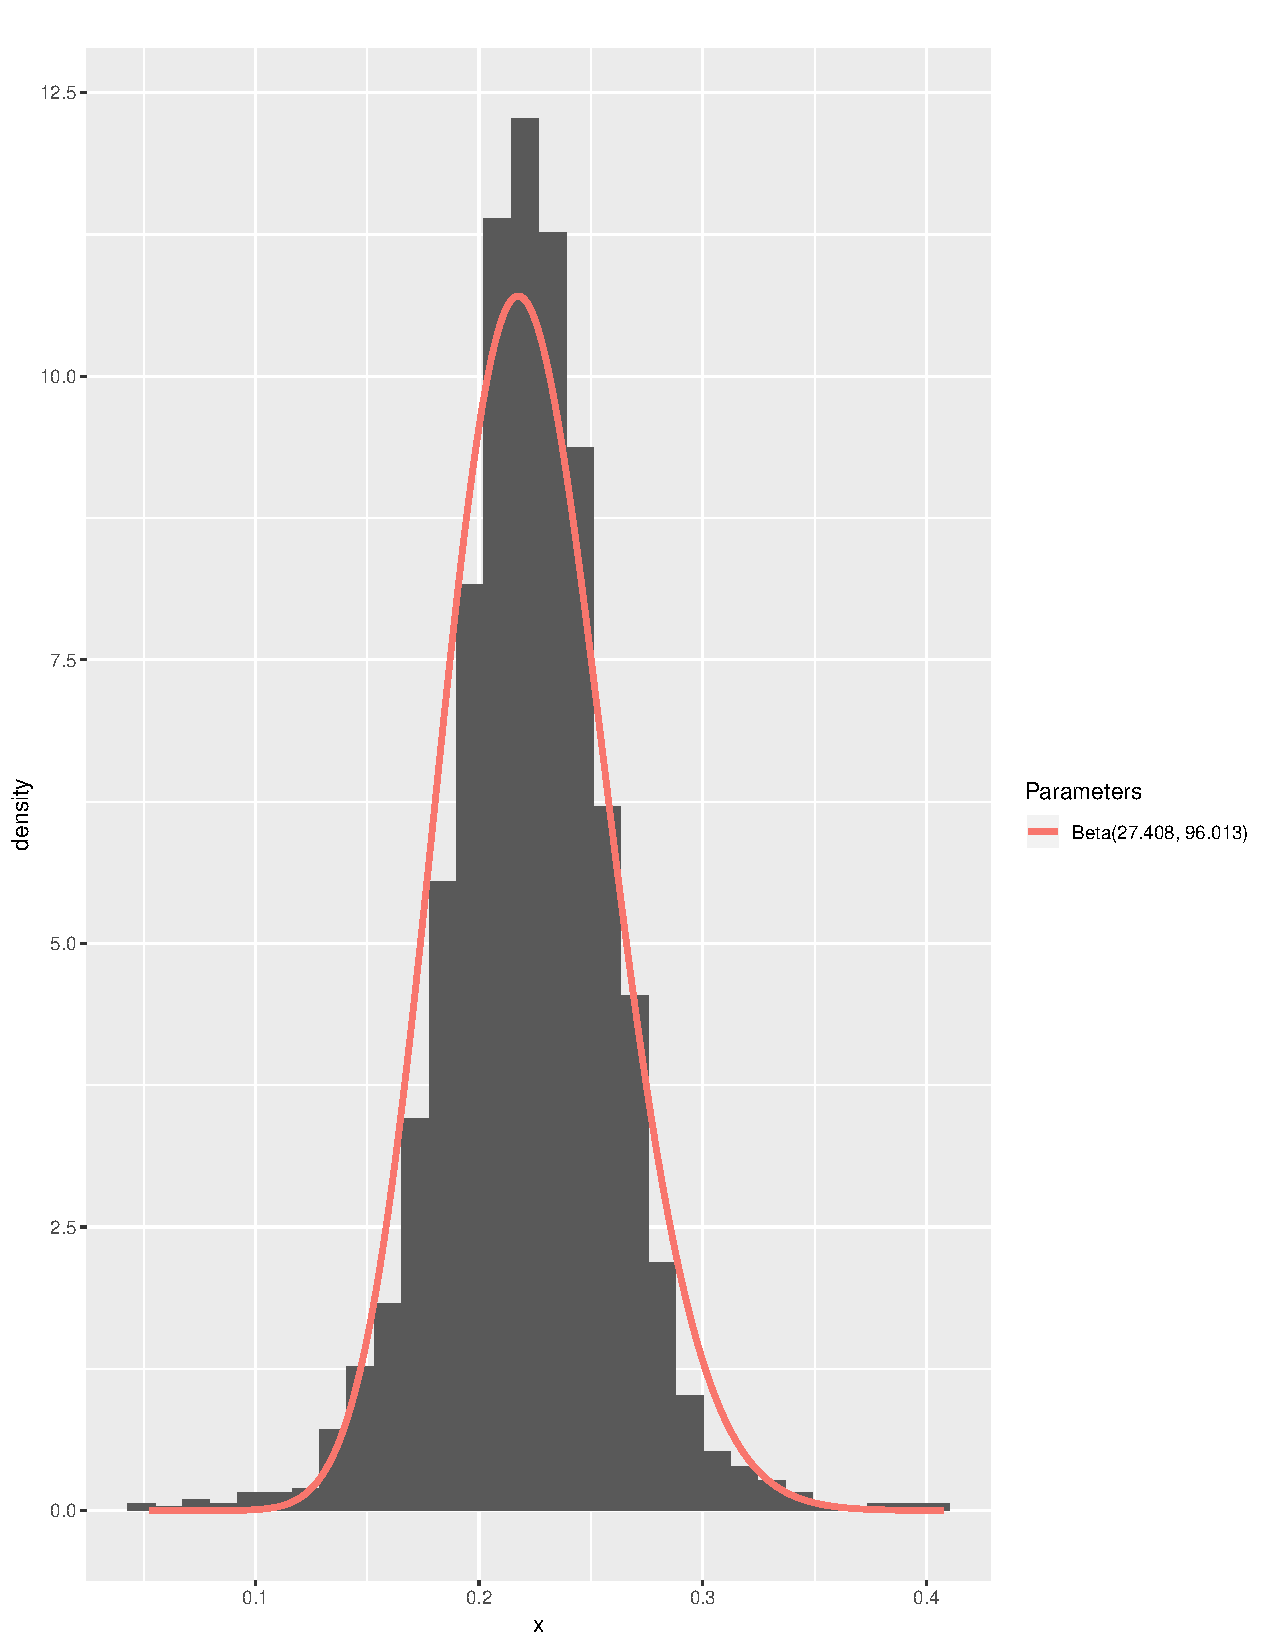
\includegraphics[width = .9\linewidth, height = .7\linewidth]{../../../Figures/paper_19_05/lh_ground.pdf}
    \caption{Similarity between PolSAR data from ground region and left helix elementary backscatterer}
    \label{fig:gr_lh}
\end{figure}

\begin{figure}[!ht]
    \centering
    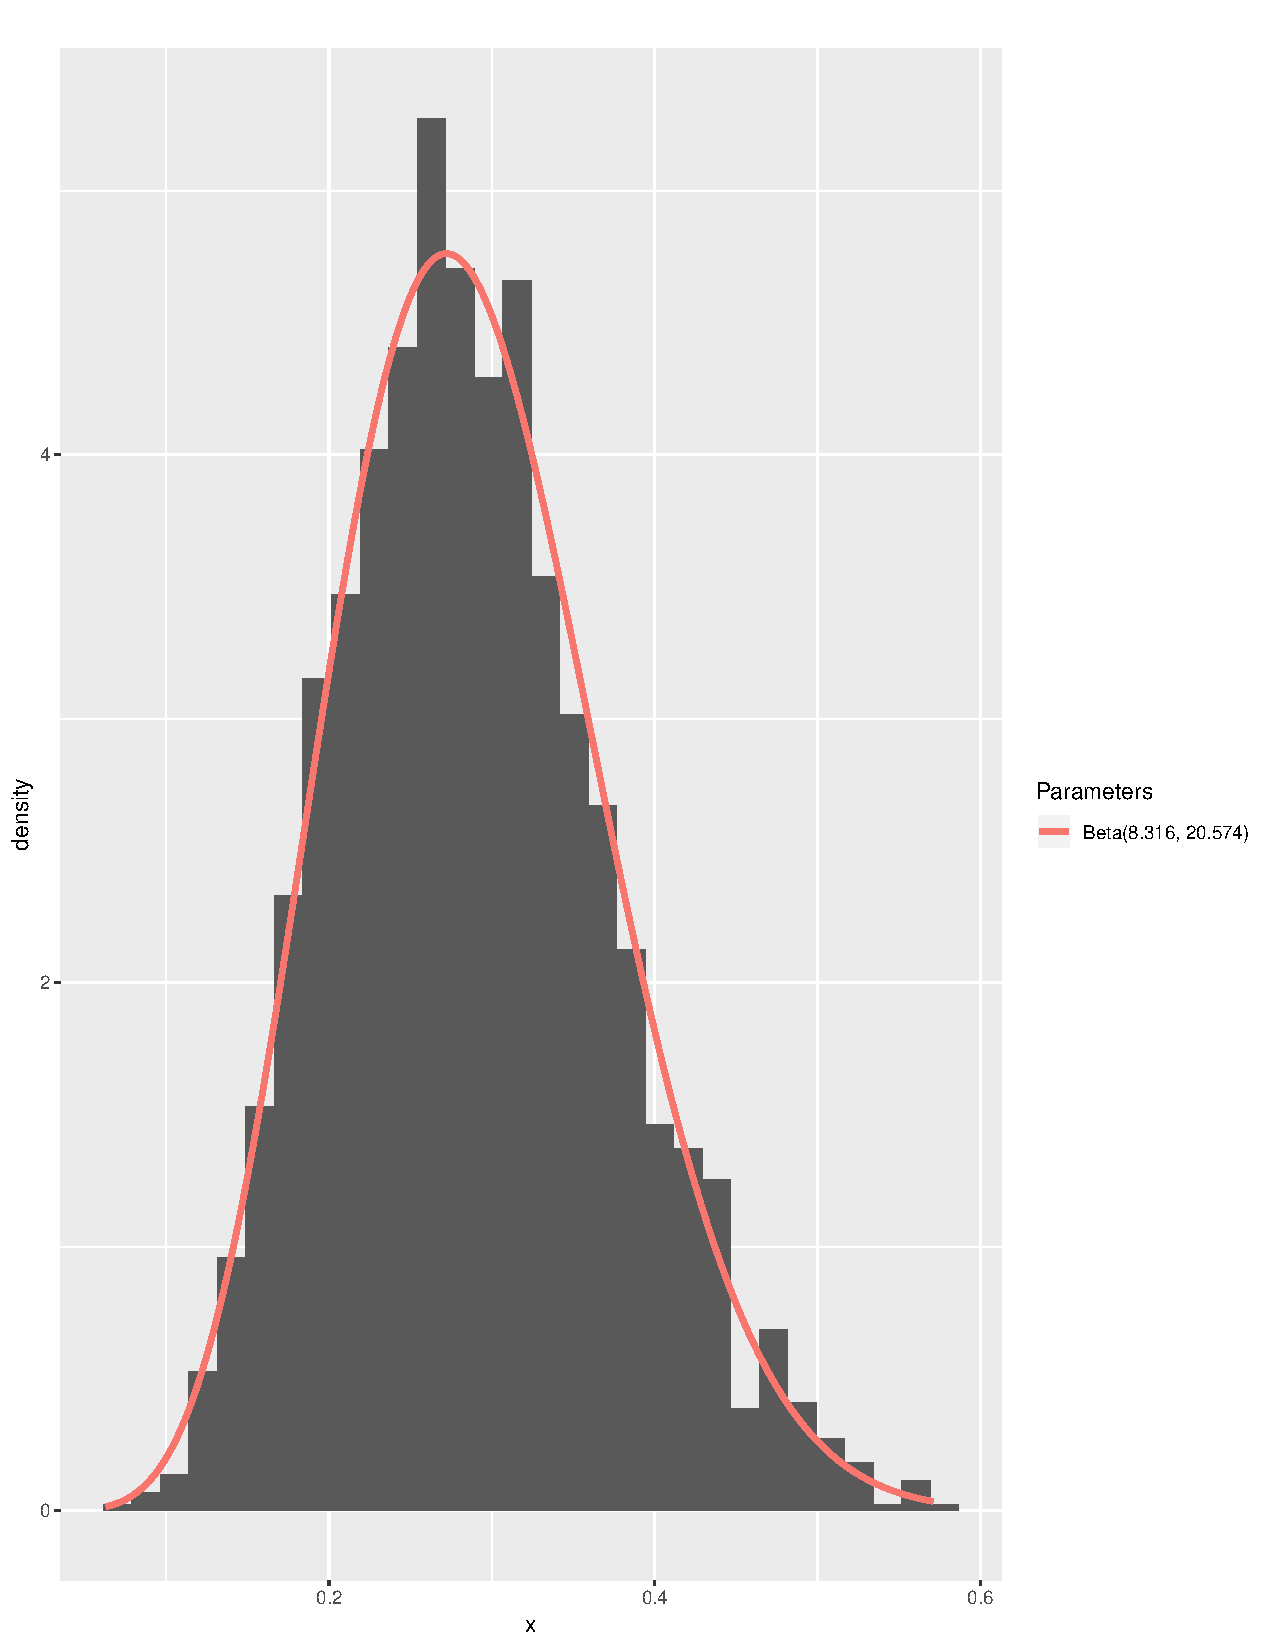
\includegraphics[width = .9\linewidth, height = .7\linewidth]{../../../Figures/paper_19_05/rh_vegetation.pdf}
    \caption{Similarity between PolSAR data from forest region and right helix elementary backscatterer}
    \label{fig:fr_rh}
\end{figure}

\begin{figure}[!ht]
    \centering
    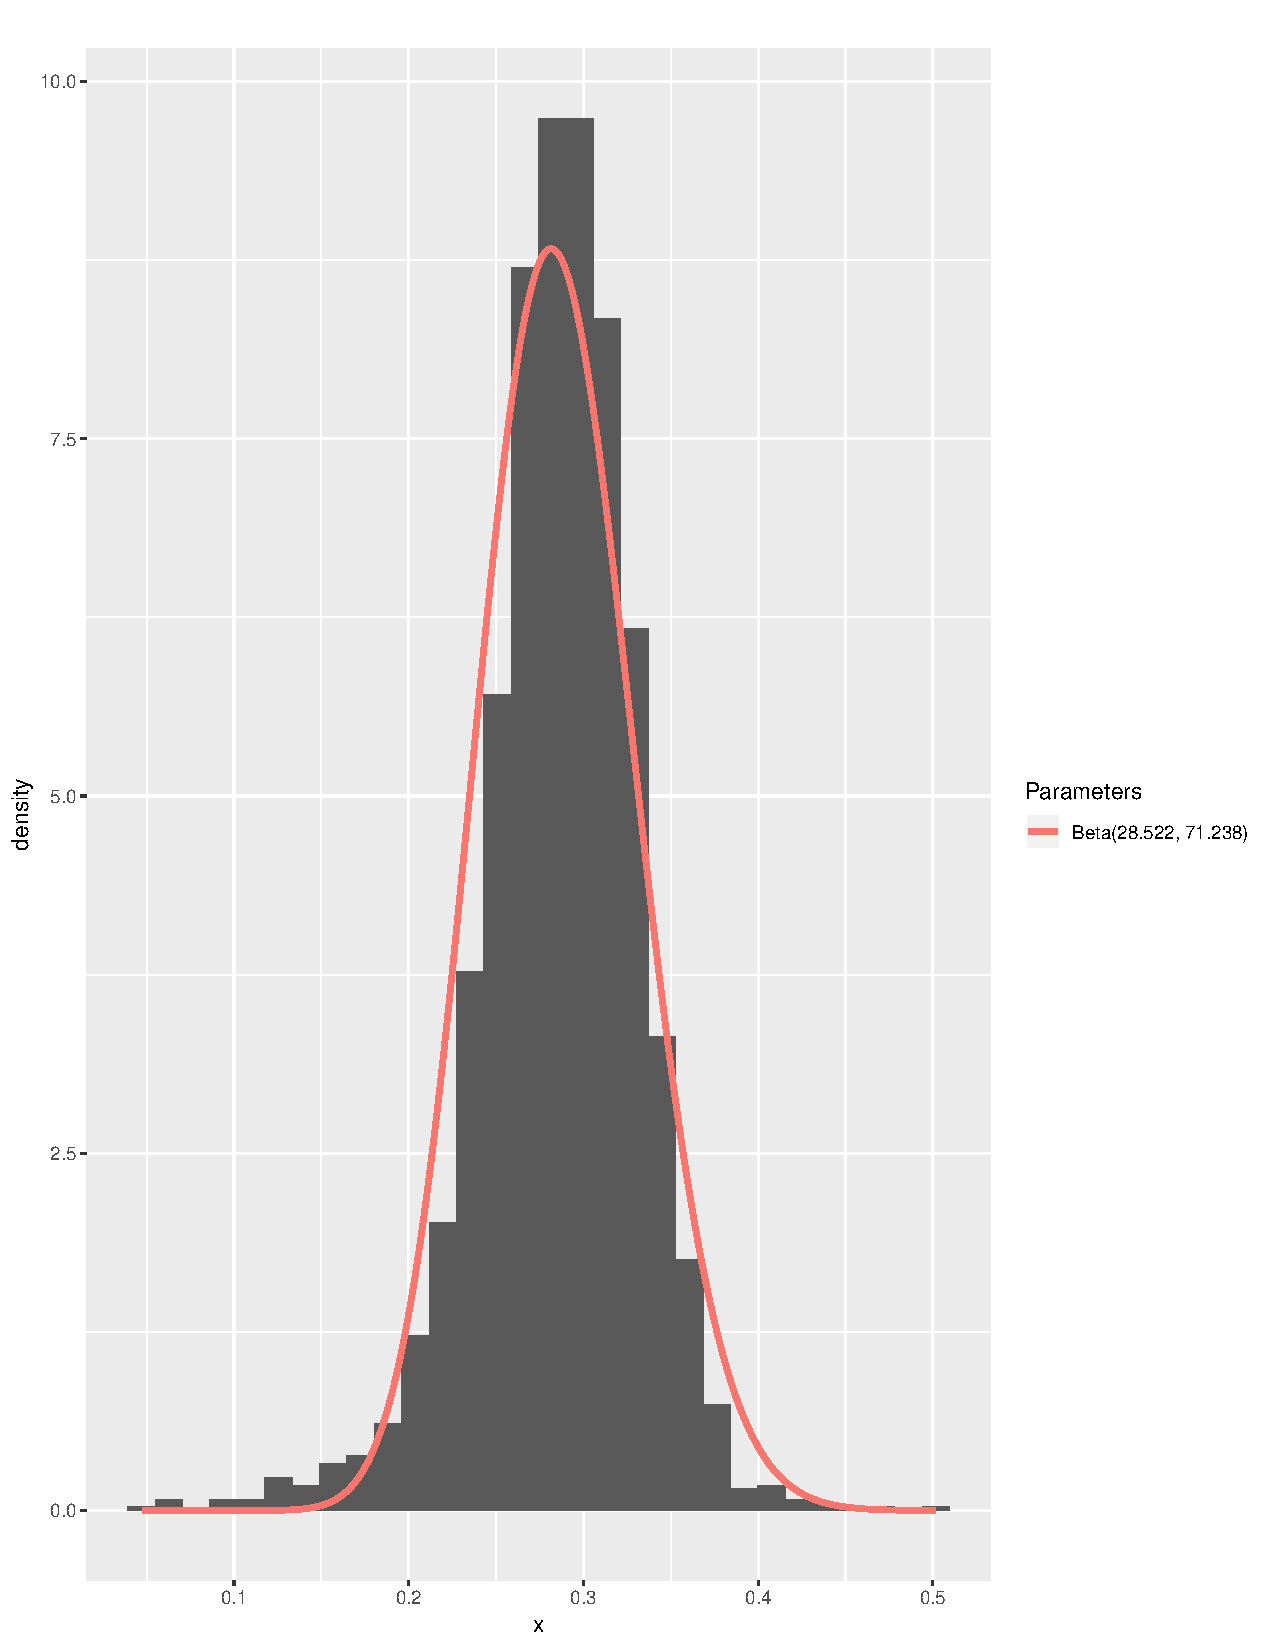
\includegraphics[width = .9\linewidth, height = .7\linewidth]{../../../Figures/paper_19_05/rh_ground.pdf}
    \caption{Similarity between PolSAR data from ground region and right helix elementary backscatterer}
    \label{fig:gr_rh}
\end{figure}

\begin{figure}[!ht]
    \centering
    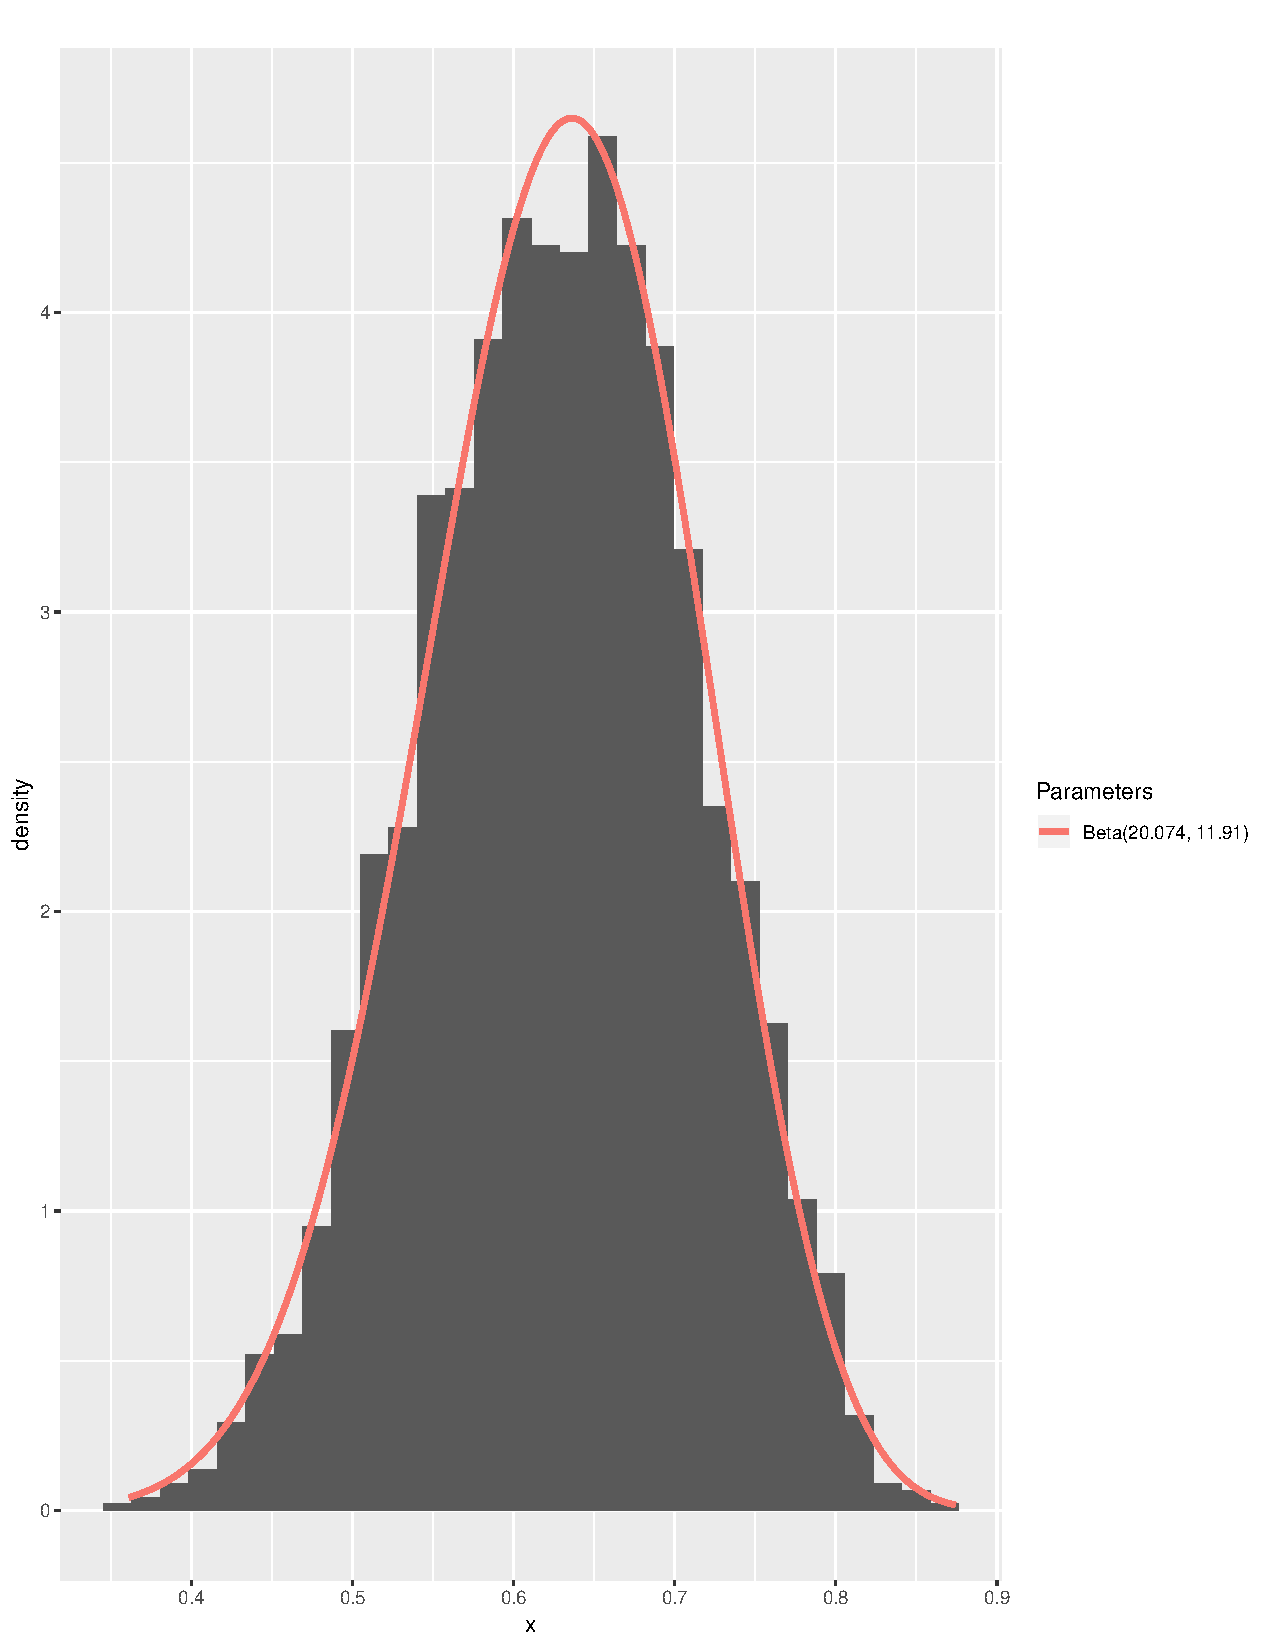
\includegraphics[width = .9\linewidth, height = .7\linewidth]{../../../Figures/paper_19_05/rv_vegetation.pdf}
    \caption{Similarity between PolSAR data from forest region and random volume elementary backscatterer}
    \label{fig:fr_rv}
\end{figure}

\begin{figure}[!ht]
    \centering
    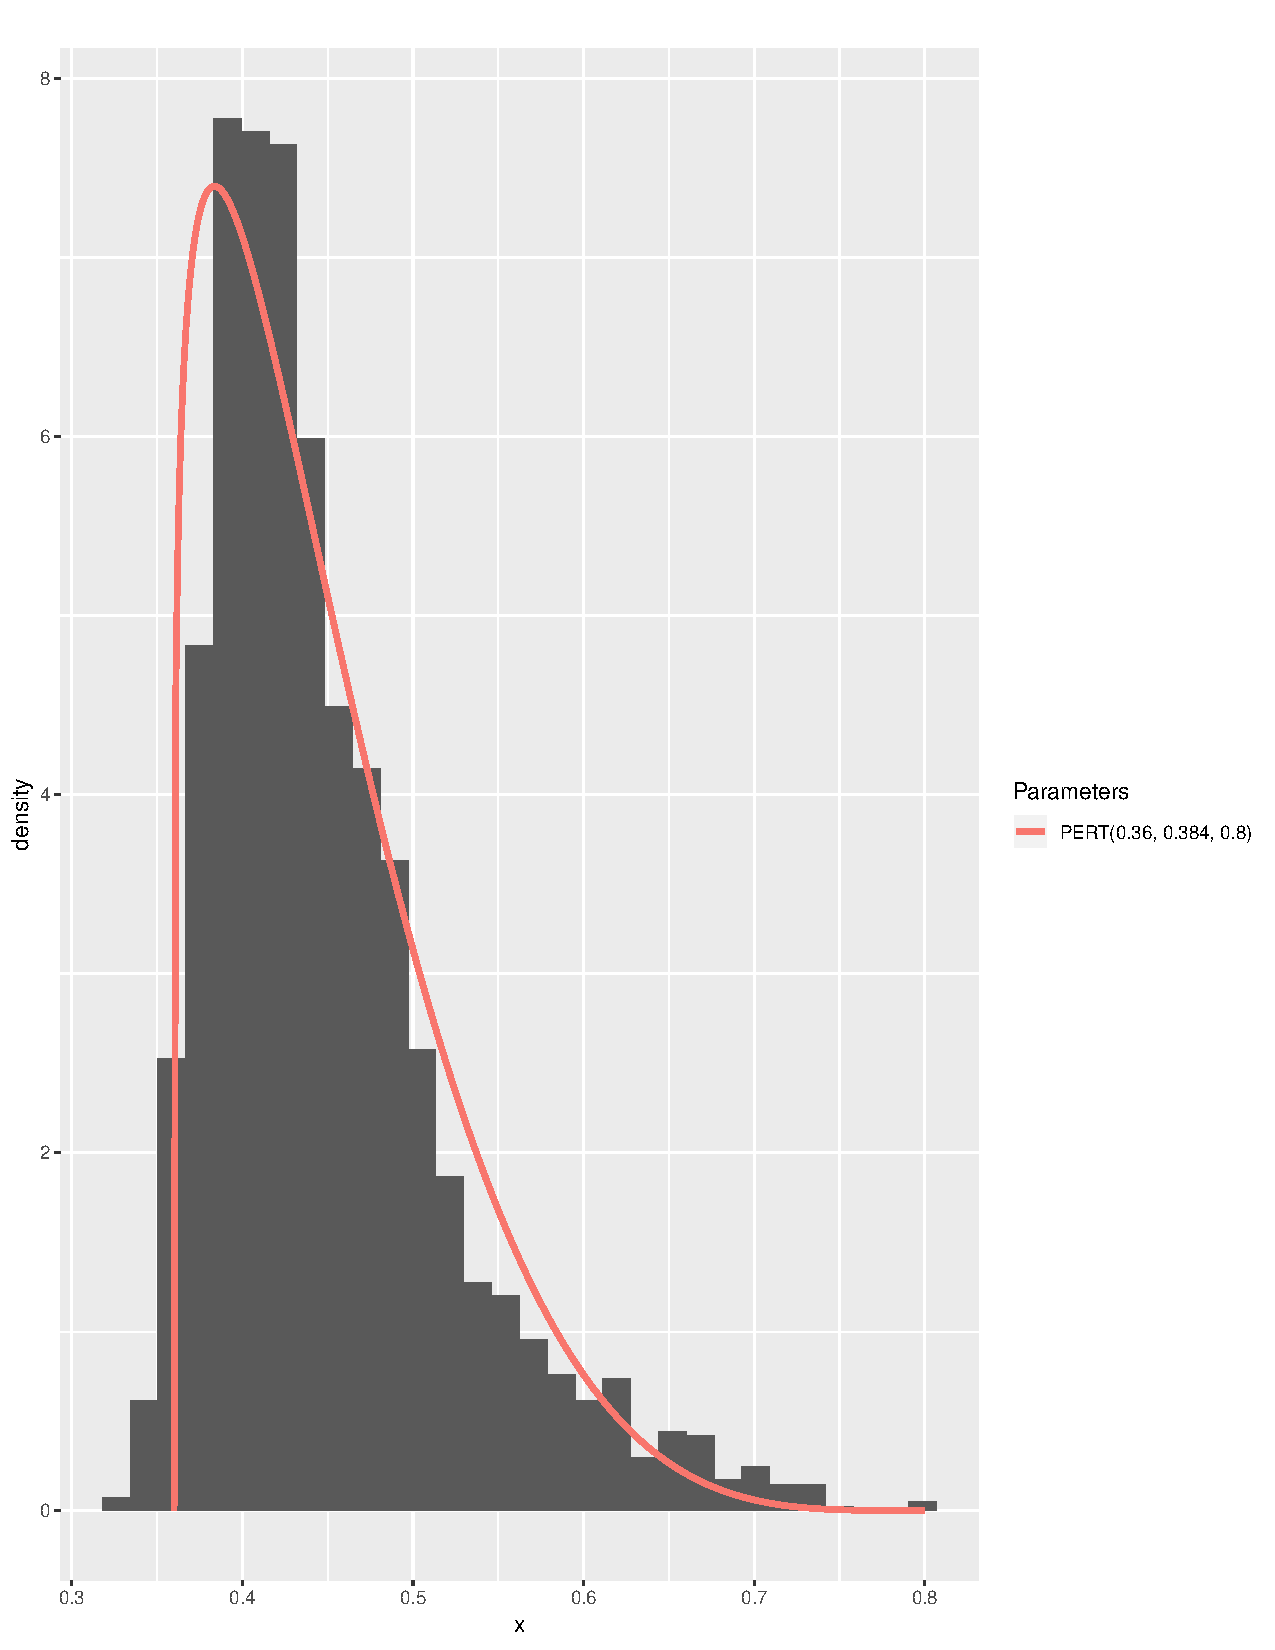
\includegraphics[width = .9\linewidth, height = .7\linewidth]{../../../Figures/paper_19_05/rv_ground.pdf}
    \caption{Similarity between PolSAR data from ground region and random volume elementary backscatterer}
    \label{fig:gr_rv}
\end{figure}

\begin{figure}[!ht]
    \centering
    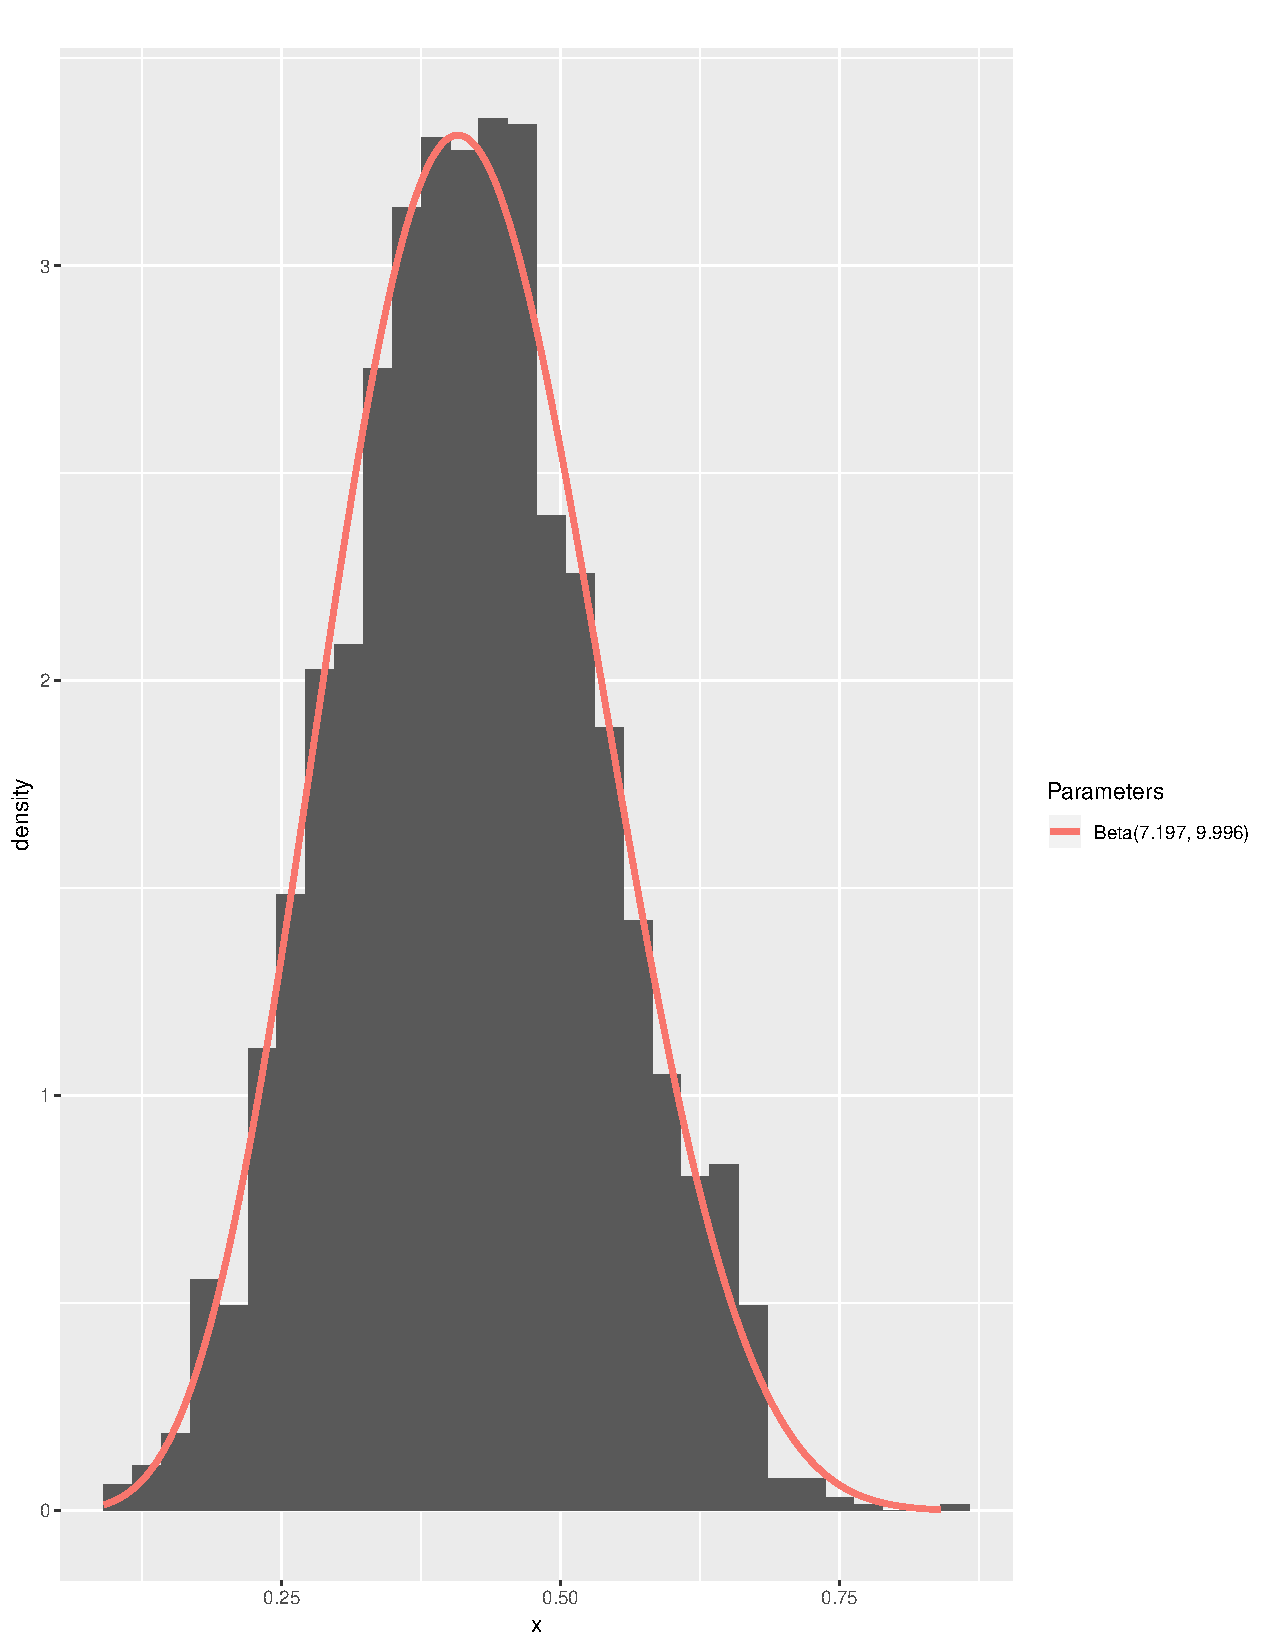
\includegraphics[width = .9\linewidth, height = .7\linewidth]{../../../Figures/paper_19_05/tr_vegetation.pdf}
    \caption{Similarity between PolSAR data from forest region and trihedral elementary backscatterer}
    \label{fig:fr_tr}
\end{figure}

\begin{figure}[!ht]
    \centering
    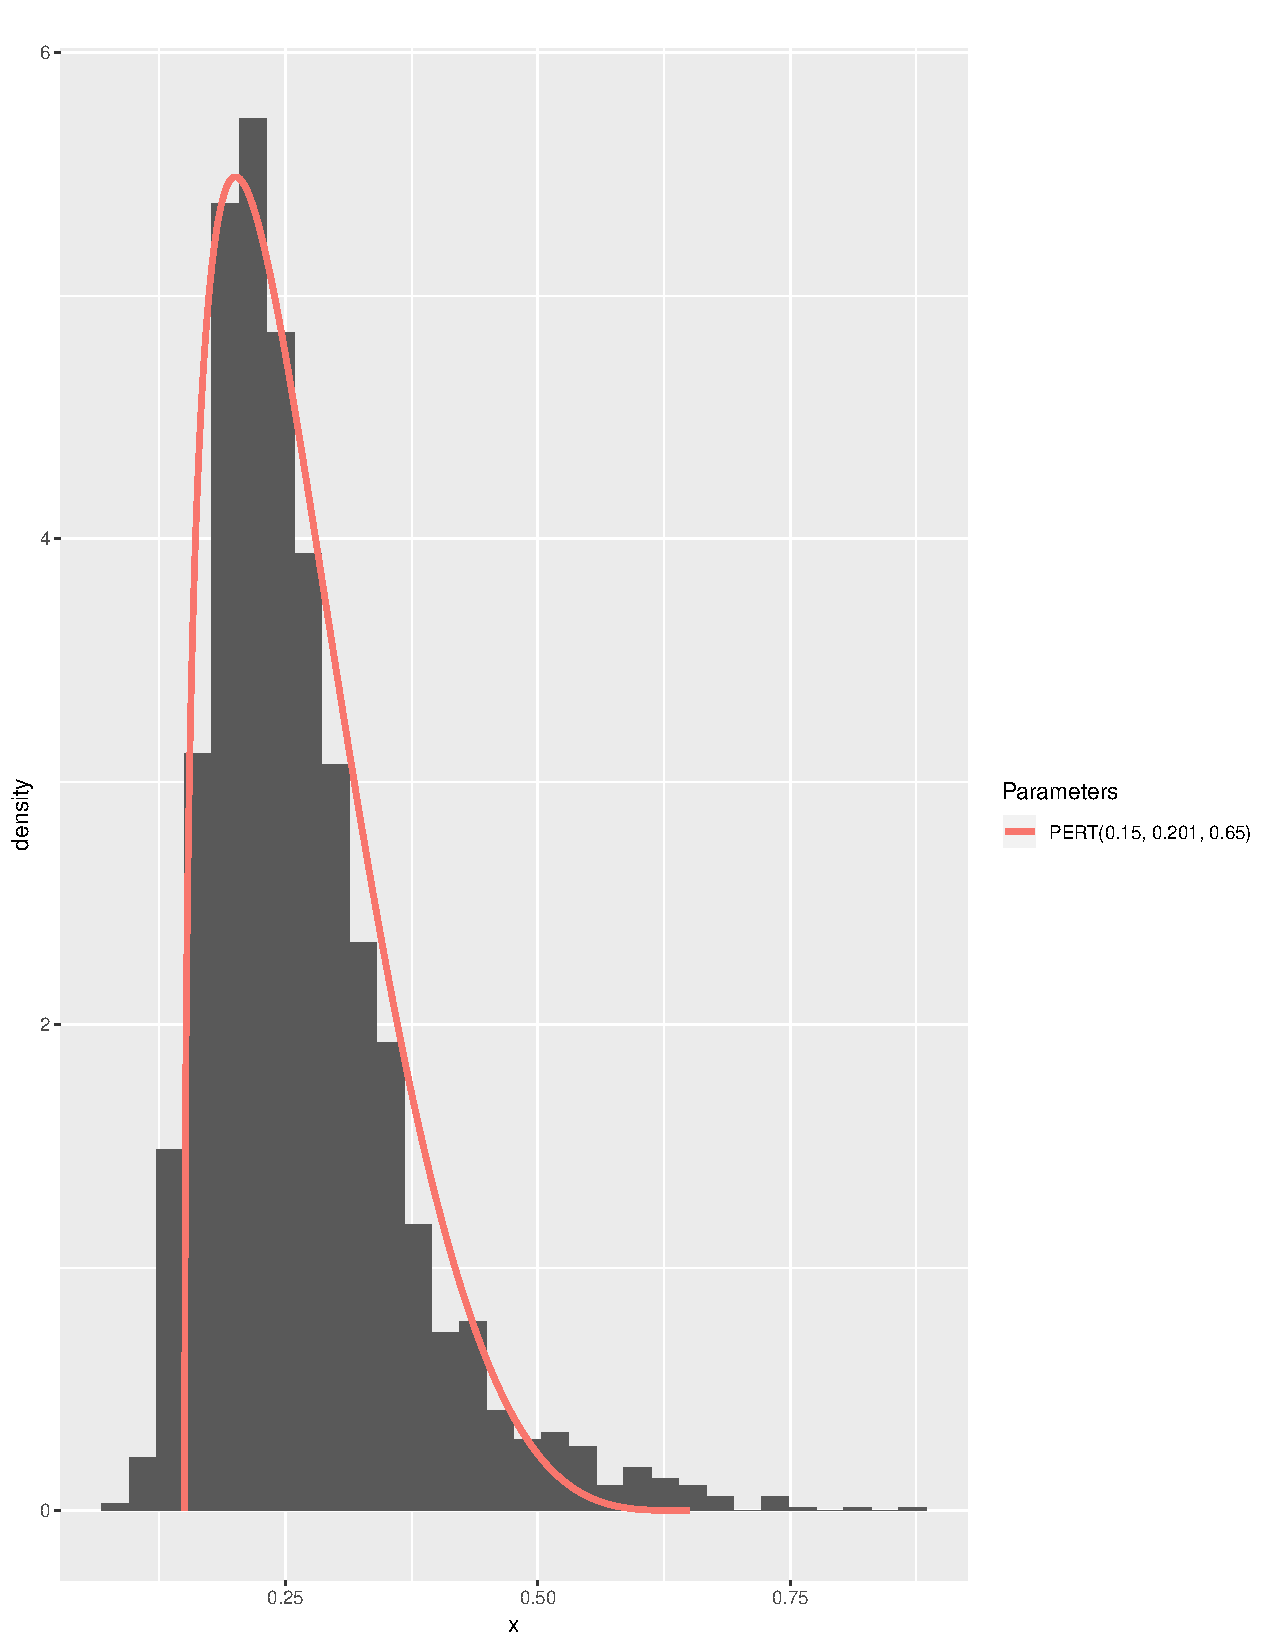
\includegraphics[width = .9\linewidth, height = .7\linewidth]{../../../Figures/paper_19_05/tr_ground.pdf}
    \caption{Similarity between PolSAR data from ground region and trihedral elementary backscatterer}
    \label{fig:gr_tr}
\end{figure}

\section{Goodness-of-fit test}

For the Kolmogorov-Smirnov goodness-of-fit test, it was selected 400 samples from the forest region and 120 samples from the ground region through simple random sampling method and realize the test for all elementary backscatterers with respect the respective distributions in the figures \ref{fig:fr_wvn} to \ref{fig:gr_tr}. The table \ref{tab:pvalues_table} contains the p-values obtained by the tests, which the least p-value is 0.07. 
\begin{table}[!ht]
\centering

    \caption{P-values obtained by Kolmogorov-Smirnov goodness-of-fit test for all elementary backscatterers}
    \label{tab:pvalues_table}     

    \begin{small}
    
        \begin{tabular}{|*{6}{p{.12\linewidth}|}}
            \hline
             & -1/4 -wave & +1/4 -wave & Cylinder & Dihedral & Dipole\\
            \hline
            \textbf{Forest} & 0.979 & 0.808 & 0.763 & 0.733 & 0.975\\
            \hline
            \textbf{Ground} & 0.361 & 0.893 & 0.264 & 0.443 & 0.475\\
            \hline
        \end{tabular} 
    \end{small} 
    \vspace{.05\linewidth}
    \begin{small}
    
        \begin{tabular}{|*{6}{p{.12\linewidth}|}}
            \hline
             & Left & Narrow & Random & Right & Trihedral\\
             & helix & dihedral & volume & helix & \\
            \hline
            \textbf{Forest} & 0.959 & 0.787 & 0.589 & 0.344 & 0.582\\
            \hline
            \textbf{Ground} & 0.099 & 0.206 & 0.480 & 0.072 & 0.127\\
            \hline
        \end{tabular} 
    \end{small} 
\end{table}

\begin{thebibliography}{00}
\bibitem{b1} D. Ratha, A. Bhattacharya, and A. C. Frery, ``Unsupervised classification of PolSAR data using
a scattering similarity measure derived
from a geodesic distance,'' IEEE Geosci. Remote Sens. Lett., vol. 15, pp. 151--155, January 2018.
\end{thebibliography}

\end{document}

